\chapter{Similarity Metrics for SQL Query Clustering}

\section{Introduction}
\label{sec:introduction}
% !TEX root = ../paper.tex
Database access logs are used in a wide variety of settings, including evaluating database performance tuning~\cite{Bruno:2005:APD:1066157.1066184}, benchmark development~\cite{pocketdata}, database auditing~\cite{kul2016ettu}, and compliance validation~\cite{Dwork2006}.
Also, many user-centric systems utilize query logs to help users by providing recommendations and personalizing the user experience~\cite{Sapia:2000:PPQ:646109.679288, giacometti2009, yang2009, stefanidis2009you, magda2010snipsuggest, chatzopoulou2011querie}. 
As the basic unit of interaction between a database and its users, the sequence of SQL queries that a user issues effectively models the user's behavior.  Queries that are similar in structure imply that they might be issued to perform similar duties. Examining a history of the queries serviced by a database can help database administrators with tuning, or help security analysts to assess the possibility and/or extent of a security breach. However, logs from enterprise database systems are far too large to examine manually. As one example, a recent study of queries at a major US bank for a period of 19 hours found nearly 17 million SQL queries and over 60 million stored procedure execution events~\cite{kul2016ettu}. Even excluding stored procedures, it is unrealistic to expect any human to manually inspect all 17 million queries per day.

Let us consider an analyst (call her Jane) faced with the task of analyzing such a query log.
Jane might first attempt to identify some interesting query fragments and their aggregate properties.
For example, she might count how many times each table is accessed or the frequency with which different classes of join predicates occur. 
Unfortunately, such fine-grained properties lack the context to clearly communicate how the data is being used, combined, and/or manipulated. 
To see the complete context, Jane must look at entire queries.
Naively, she might look at all \textit{distinct query strings} in the log.
Even comparatively small production databases typically log hundreds or thousands of distinct query strings, making direct inspection impractical.
Furthermore, it is unclear that distinct query strings are the right level of granularity in the first place.  Consider the following example queries:

{\footnotesize
\begin{enumerate}
%%%%
\item \begin{verbatim}
SELECT name FROM user
WHERE rank IN ('adm','sup')
\end{verbatim}
%%%%
\item \begin{verbatim}
SELECT SUM(balance) FROM accounts
\end{verbatim}
%%%%
\item \begin{verbatim}
SELECT name FROM user WHERE rank = 'adm'
   UNION SELECT name FROM user
         WHERE rank = 'sup'
\end{verbatim}
%%%%
\item \begin{verbatim}
SELECT SUM(accounts.balance) FROM accounts 
   NATURAL JOIN user WHERE user.rank = 'adm'
\end{verbatim}
\end{enumerate}

}

Queries 1 and 2 are clearly distinct: Their structures differ, they reference different datasets, and perform different computations. 
The remaining queries however are less so.  
Query 3 is logically equivalent to Query 1: Both compute identical results.
Conversely, although Query 4 is distinct from Queries 1 and 2, it is conceptually similar to both and shares many structural features with each.

The exact definition of similarity may depend on Jane's exact task, the content of the log, the database schema, database records, and numerous other details, some of which may not be available to Jane immediately when she first begins analyzing the log.
It is also likely that some of this information, like the precise contents of the database or even the database schema may not even be available to Jane for reasons of privacy or security.
As a result, this type of log analysis can quickly become a tedious, time-consuming process~\cite{gatterbauer2011databases}.
An earlier work of Aligon et al.~\cite{aligon2014holistic} attempted to address this problem for OLAP operations by performing query log analysis and exploration. 
Within the scope of this article, we focus on analysis of SQL queries instead of OLAP queries.
%In this article, we lay the groundwork for a more automated approach to SQL query log exploration based on hierarchical clustering.  
In particular, we lay the groundwork for a more automated approach to SQL query log exploration based on hierarchical clustering.  
Given a hierarchical clustering of the SQL query log, Jane can manually adjust how aggressively the log is summarized.
She can select an appropriate level of granularity without a \emph{priori} needing to specify exactly what constitutes a similar query.

The primary focus of this article is to study the suitability of three existing query distance metrics~\cite{aouiche2006,aligon2014similarity,makiyama2015text} to be used with hierarchical algorithms for clustering query logs. All of these metrics operate on the query structure and do not rely on the availability of underlying data or schema, thus making them applicable in a wide variety of practical settings. 
We evaluate the three metrics on two types of data: Human-authored and Machine-generated.
Thus, using an appropriate similarity metric, one can cluster the queries to obtain a meaningful clustering of the query log. %We make this measure more concrete by proposing a benchmark workload based on \textbf{d}atabase \textbf{c}ourse \textbf{a}ssignments called \dcabench.
%A common feature of many database courses is exam or homework questions where students are asked to translate english prose into SQL.  
%\dcabench evaluates queries by comparing the heuristic's clustering with this ground truth.
%For the special case of heuristics based on an inter-query distance or similarity metric, we can achieve an even more precise measure by evaluating the distance metric directly.
%\dcabench uses three statistics for evaluating distance-based clustering schemes: Silhouette Coefficient, Beta CV, and The Dunn Index.

For our evaluation, we use three evaluation data sets:
\begin{enumerate}
\item a large set of student authored queries released by IIT Bombay~\cite{chandra2015Data},
\item a smaller set of student queries gathered at 
the University at Buffalo,
%our university
and released as part of this publication, and
\item SQL logs that capture all activities on 11 Android phones for a period of one month~\cite{pocketdata}.
\end{enumerate}
Student-written queries are appealing, as queries are already labeled by their ground-truth clusterings --- For each question, the student is attempting to accomplish one specific stated task.
Conversely, machine-generated queries on smartphones present a conceptually easier challenge, as they produce more rigid, structured queries.
The three similarity metrics are evaluated on these data sets using three standard clustering evaluation statistics: Silhouette Coefficient, Beta CV, and Dunn Index~\cite{zaki2014data}. 
%The IIT Bombay dataset features a large number of distinct tasks that are individually simpler, and as a result have more overlap.
%The local exam dataset features a smaller number of harder tasks, resulting in more complex queries that are implemented through a more diverse range of query structures.
%
%We use \dcabench to evaluate three existing query distance metrics that are able to provide a pairwise similarity score from the literature~\cite{aouiche2006,aligon2014similarity,makiyama2015text}.
%Finally, we apply these similarity metrics to the bank query log that we previously mentioned, and a smartphone query log to evaluate the scalability of these metrics.
%The last bank and smartphone query logs cannot be used to evaluate the accuracy of these query similarity metrics since we do not have ground-truth information to compare with for these datasets.

None of the similarity metrics perform as well as desired, so we propose and evaluate a pre-processing step to create more regular, uniform query representations by leveraging query equivalence rules and data partitioning operations. These rules are commonly utilized by database management systems when parsing and evaluating SQL queries.
This process significantly improves the quality of all three distance metrics.
We also investigate and identify sources of errors in the clustering process. 
Experimental results show that our \emph{regularization} pre-processing technique consistently improves clustering for different query comparison schemes from the literature.

%Finally, we present a new approach to constructing distance metric based on the observation that, since SQL is a declarative language, query intent will be reflected in the query's structure and its abstract syntax tree (AST).
%The AST of a query is a tree structure that captures hierarchical relationships between elements of the query.
%For example, as seen in Figure~\ref{fig:exampleAST} the query AST's root node might have the query's Columns (i.e., Target, or SELECT), FROM, and WHERE clauses as children.  
%Our approach, based on the Weisfeiler-Lehman subgraph isomorphism algorithm, defines features based on subtrees of the AST and uses the resulting feature space to cluster queries.
%The resulting clusters are groups of queries with significantly overlapping ASTs.
%Our experiments show that this distance metric is accurate, outperforms the Aligon metric in a few respects, and establishes a promising direction for future research on query intent similarity.

%To further aid users in their understanding of query logs, we propose two techniques for summarizing and visualizing queries in a cluster: (1)  a text explanation that overviews common features of queries in the cluster, (2) a graph visualization that presents these features in the context of an actual query.

%%!TEX root = ./sections/1-intro.tex
\subsection{Motivating Application: \sysname{}}
\label{sec:motivation}
It is increasingly important for organizations to be able to detect and respond to cyber attacks.
An especially difficult class of cyber attack to detect is the so called \textit{insider attacks} that occur when employees misuse legitimate access to a resource like a database.
The difficulty arises because apparently anomalous behavior from a legitimate actor might still have legitimate intent.  
For example, a bank teller in Buffalo who withdraws a large sum for a client from California may be acting legitimately (e.g., if the client has just moved and is purchasing a house), or may be committing fraud.
The ``U.S. State of Cybercrime Survey''~\cite{cybercrimeReport2014} states that 37\% of organizations have experienced an insider incident, while a 2015 study~\cite{ponemonReport2015} identified insider attacks as having the longest average response time of any attack type surveyed: 54.5 days.

The challenge of addressing of insider attacks lies in the difficulty of precisely specifying access policies for shared resources such as databases. 
Coarse, permissive access policies provide opportunities for exploitation. 
Conversely, restrictive fine-grained policies are expensive to create and limit a legitimate actor's ability to adapt to new or unexpected tasks.
In practice, enterprise database system administrators regularly eschew fine-grained database-level access control.  
Instead, large companies commonly rely on reactive strategies that monitor external factors like network activity patterns and shared file transfers.
In a corporate environment, monitoring user actions requires less preparation and gives users a greater degree of flexibility. 
However, external factors do not always provide a strong attestation of the legitimacy of a database user's actions. 

The \sysname{}\footnote{\sysname{} is derived from the last words of the Roman emperor Julius Caesar, ``\textit{Et tu, Brute?}'' in Latin, meaning ``\textit{You, too, Brutus?}'' in English to emphasize that this system is meant to detect the unexpected betrayals of trusted people} system, currently under development at the University at Buffalo~\cite{kul2016ettu}, seeks to help analysts to monitor query access patterns for signs of insider attack.  Database logging and monitoring is expensive, so \sysname{} needs to be able to identify normal, baseline database behaviors that can be easily flagged as ``safe'' and ignored from normal logging and post-mortem attack analysis.  In this paper, we focus on one concrete part of the overall \sysname{} system, responsible for summarizing and visualizing query logs.  In the complete system, this component serves to help analysts generate patterns of safe queries, and to quickly analyze large multi-day query logs to identify potential attack activity.


%\subsection{Contributions}
Concretely, the specific contributions of this article are:
\begin{enumerate}
\item A survey of existing SQL query similarity metrics,
%\item An evaluation of these metrics on multiple query logs and a preprocessing technique for SQL queries called regularization that improves query clustering accuracy
\item An evaluation of these metrics on multiple query logs, and 
%  new benchmark and evaluation methodology for query similarity metrics,
\item Applying query standardization techniques to improve 
%our WL-based distance function, as well as functions from our survey,
query clustering accuracy. %via query standardization techniques.
%(4) A query similarity metric based on the Weisfeiler-Lehman (WL) approximate graph isomorphism algorithm~\cite{WL2011} as a promising direction. 
\end{enumerate}
%Experimental results show that our naive distance function not only mirrors intuitive notions of similarity as well as others, but has performance competitive with similar clustering techniques from the literature.

This article is organized as follows.
We start by performing a literature survey on log clustering and SQL query similarity in Section~\ref{sec:background}.
We describe a feature engineering technique called regularization in Section~\ref{sec:system}.
%In Section~\ref{sec:dcabench}, we evaluate the accuracy and performance of query similarity evaluation techniques.
In Section~\ref{sec:dcabench}, we explain our query workloads and propose a strategy for evaluating the quality of query similarity metrics.
The evaluation is presented in Section~\ref{sec:experiment}.
%, and propose a new similarity metric in Section~\ref{sec:WL}.
We discuss our experiment results, findings and ideas to further build upon the surveyed techniques in Section~\ref{sec:discussion}, and in Section~\ref{sec:scenarios}, we explain how this work can be beneficial by giving real life examples.
%and~\ref{sec:summarization}, respectively. 
Finally, we conclude by identifying the steps needed to deploy query log clustering into practice using the techniques evaluated in this article in Section~\ref{sec:conclusion}.

%The focus of this paper is to model user intents via query monitoring. Provided that an accurate model can be created, it would lead not only to effective insider attack detection systems, but could have implications for other fields like database performance optimizers.



\section{Background}
\label{sec:background}
% !TEX root = ../paper.tex

Analyzing query logs mostly relies on the structure of queries~\cite{Kamra2007SyntaxBased}, although their motivations are different; some methods prefer using the log as a resource to collect information to build user profiles, and the others utilize structural similarity to perform tasks like query recommendation~\cite{giacometti2009, yang2009, chatzopoulou2011querie}, performance optimization~\cite{aouiche2006},  session identification~\cite{aligon2014similarity} and workload analysis~\cite{makiyama2015text}.  A summary of these methods is given in Table~\ref{table:literaturereview}.

There are also other possible approaches; like data-centric query comparison~\cite{Mathew2010Raid}, and utilizing the \textit{access areas} of user queries by inspecting the data partition the query is interested in~\cite{nguyen2015identifying} from the \texttt{WHERE} condition.
However, these approaches are out of our scope
since we are interested in comparing and improving methods based on structural similarity; we assume that
we do not have access to the data or the statistical information about the database. 

\begin{table*}[h]
\centering
\begin{tabular}{ C{3.8cm}  C{2.9cm}  C{3.9cm}  C{1.15cm}  C{2.65cm} C{1.35cm}}
\toprule
Paper title & Motivation & Features & Feature Structure & Distance Function & Similarity Ratio \\
\midrule
Agrawal \textit{et al.} (2006)~\cite{agrawal2006context} & Q. reply importance & {\footnotesize Schema, rules} & Vector & Cosine similarity & No \\
Giacometti \textit{et al.} (2009)~\cite{giacometti2009} & Q. recommendation & {\footnotesize Difference pairs} & Set  & Difference query  & No \\[-1mm]
Yang \textit{et al.} (2009)~\cite{yang2009} & Q. recommendation & {\footnotesize Selection/join, projection} & Graph & \parbox{2.6cm}{\footnotesize \center Jaccard coefficient\\[-0.5mm] on the graph edges} & No \\
Stefanidis \textit{et al.} (2009)~\cite{stefanidis2009you} & Data Recommendation & {\footnotesize Inner product of two queries} & Vector & - &  No \\
Khoussainova \textit{et al.} (2010)~\cite{magda2010snipsuggest} & Q. recommendation & {\footnotesize Popularity of each query object} & Graph & -  & No \\[-1mm]
Chatzopoulou \textit{et al.} (2011)~\cite{chatzopoulou2011querie} & Q. recommendation & {\footnotesize Syntactic element frequency} & Vector & \parbox{2.65cm}{\footnotesize \center Jaccard coefficient\\[-0.5mm]and cosine similarity} & No  \\
Aouiche \textit{et al.} (2006)~\cite{aouiche2006} & View selection & {\footnotesize Selection/join, group-by} & Vector & Hamming distance  & Yes \\
Aligon \textit{et al.} (2014)~\cite{aligon2014similarity} & Session similarity & {\footnotesize Selection/join, projection, group-by} & 3 Sets & Jaccard coefficient   & Yes \\
Makiyama \textit{et al.} (2016)~\cite{makiyama2015text} & Workload analysis & {\footnotesize Term frequency of projection, selection/join, from, group-by and order-by} & Vector & Cosine similarity  & Yes \\
\bottomrule
\end{tabular}
\vspace*{-2mm}
\caption{SQL query similarity literature review}
\label{table:literaturereview}
\end{table*}

Agrawal \textit{et al.}~\cite{agrawal2006context} aim to rank the tuples returned by the SQL query based on the context.
They create a ruleset for contexts and evaluate the result of queries that belongs to the context according to the ruleset.
They capture context and query as feature vectors and capture similarity through cosine distance between the vectors.

Chatzopoulou \textit{et al.}~\cite{chatzopoulou2011querie} aim to assist non-expert users of scientific databases by tracking their querying behavior and generating personalized query recommendations.
They deconstruct an SQL query into a bag of \textit{fragments}.
Each distinct fragment is a feature, with a weight assigned to it indicating its importance.
Each feature has two types of importance: (1) within the query and (2) for the overall workload.
Similarity is defined upon common vector-based measures such as cosine similarity.
A summarization/user profile for this approach is just a sum over all single query feature vectors that belong to their workload.

Yang \textit{et al.}~\cite{yang2009}, on the other hand, build a graph following
the query log by connecting associations of table attributes from the input and output of queries which are then used to compute the likelihood of an attribute appearing in a query with a similarity function like Jaccard coefficient.
Their aim is again to assist users in writing SQL queries by analyzing query logs. Giacometti \textit{et al.}~\cite{giacometti2009}, similarly, aim to make recommendations on the discoveries made in the previous sessions for users to spend less time on investigating similar information.
They introduce \textit{difference pairs} in order to measure the relevance of the previous discoveries.
Difference pairs are essentially the result columns that is not included in the other return results; hence the method depends on having access to the data.
Stefanidis \textit{et al.}~\cite{stefanidis2009you} takes a different approach, and instead of recommending candidate queries, they recommend tuples that may be of interest to the user.
By doing so, the users may decide to change the selection criteria of their queries in order to include these results.

Sapia~\cite{Sapia:2000:PPQ:646109.679288} creates a model that learns query templates to prefetch data in OLAP systems based on the user's past activity. SnipSuggest~\cite{magda2010snipsuggest}, on the other hand, is a context-aware SQL-autocomplete system that helps database users to write SQL queries by suggesting SQL snippets.
In particular, it assigns a probability score to each subtree of a query based on the subtree's frequency in a query log.
These probabilities are used to discover the most likely subtree that a user is attempting to construct, at interactive speeds.

Although these methods~\cite{agrawal2006context, chatzopoulou2011querie, yang2009, giacometti2009, stefanidis2009you, magda2010snipsuggest} utilize query similarity one way or other to achieve their purpose, they don't directly offer a way to compare query similarity. 
We aim to summarize the log and the most practical way to describe a query log is to group similar queries together so that we can provide summaries of these groups to the users.
For this purpose, we need to be able to measure pairwise similarity between each query, hence we need a metric that can do so. As shown in Table~\ref{table:literaturereview}, this condition is only satisfied by \cite{aouiche2006, aligon2014similarity, makiyama2015text}.

Aouiche \textit{et al.}~\cite{aouiche2006} is the first work we encountered that proposes a pairwise similarity metric between two SQL queries although it is not the aim of their work.
They aim to optimize view selection in warehouses by the queries posed to the system.
They consider the \textit{selection}, \textit{joins} and \textit{group-by} items in the query to create vectors and use Hamming Distance to measure how similar two queries are.
While creating the vector, it doesn't matter if an item appears more than once or where the item is.
They cluster similar queries that creates a workload on the system and base their view creation strategy in the system on the clustering result. 

Aligon \textit{et al.}~\cite{aligon2014similarity} study various approaches to defining a similarity function to compare OLAP sessions.
They focus on comparing session similarity while also performing a survey on query similarity metrics.
They identify \textit{selection} and \textit{join} items as the most relevant components in a query followed by the \textit{group by} set.
Inspired by the findings, they propose their own query similarity metric which considers \textit{projection}, \textit{group-by}, \textit{selection-join} items for queries issued on OLAP datacubes. 
OLAP datacubes are multidimensional models, and they have hierarchy levels for the same attributes. Aligon \textit{et al.}~\cite{aligon2014similarity} measure the distance between the attributes on different hierarchy levels, and compute the set similarity for \textit{projection}, \textit{group-by}, and \textit{selection-join} sets individually when comparing two queries.
In our experiments, since we do not consider the hierarchy levels in an OLAP system but focus on databases, we consider all queries are on the same level in the schema to adjust the formulas presented in the paper. 
Namely, we compute set similarity of \textit{projection}, \textit{group-by}, \textit{selection-join} sets of two queries with Jaccard coefficient. 
Also, Aligon \textit{et al.}~\cite{aligon2014similarity} provide the flexibility to adjust weights of the three feature sets based on the domain needs. We explore how the clustering quality is affected with various weightings in Appendix~\ref{appendix:aligon}.

Makiyama \textit{et al.}~\cite{makiyama2015text} approach query log analysis with the goal of analyzing a system's workload, and they provide a set of experiments on Sloan Digital Sky Survey (SDSS) dataset.
They extract the terms in \textit{selection}, \textit{joins}, \textit{projection}, \textit{from}, \textit{group-by} and \textit{order-by} items separately and record their appearance frequency.
They create a feature vector using the frequency of these terms which they use to calculate the pairwise similarity of queries with cosine similarity.
Instead of clustering, they perform the workload analysis with Self-Organizing Maps (SOM).

To further illustrate how the three structural metrics~\cite{aouiche2006, aligon2014similarity, makiyama2015text} work, we show the feature representations for the following query for each method in Table~\ref{tab:features}.
{\footnotesize
\begin{verbatim}
SELECT u.username, u.yearenrolled
FROM user u, accounts a
WHERE u.id = a.userid
  AND a.balance > 1000
  AND u.id > 20050001
GROUP BY u.yearenrolled
ORDER BY u.yearenrolled
\end{verbatim}
}

\begin{table}[]
\centering

\begin{tabular}{C{2cm}  l}
\toprule

        Paper title & \multicolumn{1}{c}{Extracted Feature Vector}                                                                                                                                                                                                                                                                                                                                               \\ \midrule
Aouiche \textit{et al.} (2006)~\cite{aouiche2006}  & \begin{tabular}[c]{@{}l@{}}\{`u.id', `a.userid', `a.balance',  `u.yearenrolled'\}\end{tabular}                                                                                                                                                                                                                                                                                                   \\ \midrule
Aligon \textit{et al.} (2014)~\cite{aligon2014similarity}   & \begin{tabular}[c]{@{}l@{}}\{`u.username`, `u.yearenrolled'\}\\ \{`u.id', `a.userid', `a.balance'\}\\ \{`u.yearenrolled'\}\end{tabular}                                                                                                                                                                                                                                                                \\ \midrule
Makiyama \textit{et al.} (2016)~\cite{makiyama2015text} & \begin{tabular}[c]{@{}l@{}}\{`SELECT\_u.username' \textrightarrow 1,\\  `SELECT\_u.yearenrolled' \textrightarrow 1,\\   `FROM\_user \textrightarrow 1', `FROM\_accounts' \textrightarrow 1,\\   `WHERE\_u.id' \textrightarrow 2, `WHERE\_a.userid' \textrightarrow 1,\\ `WHERE\_a.balance' \textrightarrow 1,\\   `GROUPBY\_u.yearenrolled' \textrightarrow 1,\\   `ORDERBY\_u.yearenrolled' \textrightarrow 1\}\end{tabular} \\ 
\bottomrule
\end{tabular}
\vspace*{-2mm}
\caption{Representation of three similarity metrics}
\label{tab:features}
\end{table}

In the next section, we propose a generalized feature engineering scheme for query comparison methods to improve the clustering quality.
Our work evaluates the performance of the three methods~\cite{aouiche2006, aligon2014similarity, makiyama2015text} that directly describe a pairwise similarity metric in Section~\ref{sec:dcabench} due to the lack of performance evaluation for the query similarity metrics in the given studies.
We also show that our feature engineering scheme improves the clustering quality with both statistical and empirical methods.

\section{Feature Engineering}
\label{sec:system}
% !TEX root = ../paper.tex
The grammar of SQL is declarative. By design, users can write queries in the way they feel most comfortable, letting well-established equivalence rules dictate a final evaluation strategy.  As a result, many syntactically distinct queries may still be semantically equivalent.  Recall example queries 1 and 3, paraphrased here:

{\footnotesize
\begin{enumerate}
\item\begin{verbatim}
SELECT name FROM user 
WHERE rank = 'a' OR rank='s'
\end{verbatim}
\stepcounter{enumi}
\item\begin{verbatim}
SELECT name FROM user WHERE rank = 'a'
UNION SELECT name FROM user WHERE rank = 's'
\end{verbatim}
\end{enumerate}
}

Though semantically distinct, these queries produce identical results for any input.  Unfortunately similarity of results is not practical to implement: General query equivalence is NP-complete~\cite{Chandra:1977:OIC:800105.803397} for SQL92 and earlier, while SQL99 and later versions of SQL are turing-complete, due to the introduction of recursive queries.  

However, we can still significantly improve clustering quality by standardizing certain SQL features into a more regular form with techniques such as canonicalizing names and aliases, removing syntactic sugaring, and standardizing nested query predicates.
This process of \emph{regularization} aims to produce a new query that is more likely to be \emph{structurally} similar to other \emph{semantically} similar queries. 
Because the output is an ordinary SQL query, regularization may be used with any similarity metric.
These process is similarly used in~\cite{Chandra:2016:PMA:3007263.3007304, sapia1999modeling}, where Chandra~\textit{et al.}~\cite{Chandra:2016:PMA:3007263.3007304} generate mutations of SQL queries to catch diversions from a baseline query, and Sapia~\cite{sapia1999modeling} creates OLAP query prototypes based on selected features and models user profiles.


Although the techniques we utilize for regularization are widely used in other settings, to the best of our knowledge, we introduce their usage to improve clustering quality.
We also test all the techniques we use individually to find their impact on the regularization's overall effect.
Our experiments in Section~\ref{subsec:evaluation} show consistent improvements for all metrics evaluated in practical real world settings.
In this section, we describe the transformations that we apply to regularize queries and the conditions under which they may be applied.  

\subsection{Regularization Rules}
\label{sec:regularizationrules}

\tinysection{Canonicalize Names and Aliases}
As we will show in our experiments in Section~\ref{sec:experiment}, table and attribute aliases are a significant source of error in matching. Consider the following two queries:

{\footnotesize
\begin{enumerate}
\addtocounter{enumi}{4}
\item\begin{verbatim}
SELECT name FROM user
\end{verbatim}
\item\begin{verbatim}
SELECT id 
FROM (SELECT name AS id FROM user) AS t
\end{verbatim}
\end{enumerate}
}

Although these queries are functionally identical, variable names are aliased in different ways.  This is especially damaging for the three structural heuristics that we evaluate, each of which assumes that variable names follow a globally consistent pattern.  Our first regularization step attempts to create a canonical naming scheme for both attributes and tables which is similar to one used in \cite{Chandra:2016:PMA:3007263.3007304}.

\begin{table}
\centering
\begin{tabular}{C{2.5cm}| C{5cm}}
\textbf{Before}  & \textbf{After} \\
\hline
$b\; \{>, \geq\}\; a$ & $a\; \{<, \leq\}\; b$\\
{\footnotesize x \textbf{BETWEEN} (a,b)}   & $a\leq x$ \textbf{AND} $x\leq b$\\
 x \textbf{IN} ($a$,$b$,\ldots) &  x=$a$ \textbf{OR} x=$b$ \textbf{OR} \ldots\\
 isnull(x,y)  &\textbf{CASE WHEN} x is null \textbf{THEN} y \textbf{END}          \\
\end{tabular}
\caption{Syntactic Desugaring}
\label{table:syntacticsugar}
\vspace*{-5mm}
\end{table}

\tinysection{Syntax Desugaring}
We remove SQL's redundant syntactic sugar following basic pattern-replacements as shown in Table~\ref{table:syntacticsugar}.  

\tinysection{EXISTS Standardization}
Although SQL admits four classes of nested query predicates: (\texttt{EXISTS}, \texttt{IN}, \texttt{ANY}, and \texttt{ALL}), the \texttt{EXISTS} predicate is general enough to capture the semantics of the remaining operators~\cite{Chandra:2016:PMA:3007263.3007304}.  Queries using the others are rewritten:\\
\noindent \texttt{x IN (SELECT y \ldots)} \textbf{becomes} \\\hspace*{22.5mm}\texttt{EXISTS (SELECT * \ldots WHERE x = y)}\\
\noindent \texttt{x $<$ ANY (SELECT y \ldots)} \textbf{becomes}  \\\hspace*{22.5mm}\texttt{EXISTS (SELECT * \ldots WHERE x $<$ y)}\\
\noindent \texttt{x $<$ ALL (SELECT y \ldots)} \textbf{becomes}  \\\hspace*{14.5mm}\texttt{NOT EXISTS (SELECT * \ldots WHERE x $\geq$ y)}

\tinysection{DNF Normalization}
We normalize all boolean-valued expressions by converting them to disjunctive normal form (DNF).  The choice of DNF is motivated by the ubiquity of conjunctive queries in most database applications, as well as by the natural correspondence between disjunctions and unions that we exploit below.

\tinysection{Commutative Operator Ordering}
We standardize the order of expressions involving commutative and associative operators (e.g., $\wedge$, $\vee$, $+$, and $\times$) by defining a canonical order of all operands and traversing the expression tree bottom-up to ensure consistent order of all operands.

%\smallskip

\tinysection{Flatten FROM-Nesting}
We merge nested sub-queries in a \texttt{FROM} clause with its parent query as described in \cite{Chandra:2016:PMA:3007263.3007304}.

\tinysection{Nested Query De-correlation}
A common database optimization called nested-query de-correlation~\cite{492194} converts some \texttt{EXISTS} predicates into joins for more efficient evaluation. 
Note that this rewrite does not guarantee query result equivalence under \textit{bag semantics} due to duplicated rows in the result.
Hence we require that the parent query is either a \texttt{SELECT DISTINCT} or a duplicate-insensitive aggregate~\cite{ilprints101} (e.g. $max\{1,1\}=max\{1\}$, but $sum\{1,1\}\neq sum\{1\}$).
If the \texttt{EXISTS} predicate is in a purely conjunctive \texttt{WHERE} clause, the de-correlation process simply moves the query nested in the \texttt{EXISTS} into the \texttt{FROM} clause of its parent query. 
The (formerly) nested query's \texttt{WHERE} clause can be then merged into the parent's \texttt{WHERE} clause. 
Specifically, if the input query is of the form:

{\footnotesize
\begin{verbatim}
SELECT ... FROM R WHERE 
           EXISTS (SELECT ... FROM S WHERE q)
\end{verbatim}
}

then the output query will have the form:

{\footnotesize
\begin{verbatim}
SELECT ... FROM R, (SELECT ... FROM S) WHERE q
\end{verbatim}
}

To de-correlate a \texttt{NOT EXISTS} predicate, we use the set-difference operator \texttt{EXCEPT}.  If the input is of the form:
{\footnotesize
\begin{verbatim}
SELECT DISTINCT... FROM R WHERE 
       NOT EXISTS (SELECT ... FROM S WHERE q)
\end{verbatim}
}
then the output will be of the form
{\footnotesize
\begin{verbatim}
(SELECT DISTINCT... FROM R) EXCEPT 
  (SELECT DISTINCT... FROM R, WHERE 
           EXISTS (SELECT ... FROM S WHERE q))
\end{verbatim}
}
%Ignoring EXISTS temporarily and one would get\begin{definition}
%Pre-filter query (PFQuery):
%The resulting query generated by replacing one of its boolean expressions that contains a sub-query with a tautology. 

%Pre-filtered output (PFOut):
%Output of PFQuery.
%\end {definition}

%In cases that attributes that belong to PFOut(before PROJECTION) appear in sub-query.
%\begin{definition}
%Correlated attributes:
%Attributes belonging to PFOut that appear in filtering predicates of sub-query.
%\end{definition}

%Below gives a simple example of correlated attributes.\begin{example}
%\begin{verbatim}SELECT A.a FROM A WHERE A.a<1 AND 
%EXISTS(SELECT * FROM B WHERE B.b=A.b)
%\end{verbatim}
%\end{example}
%Predicate B.b=A.b correlates PFQuery with sub-query in EXISTS by the correlated attribute A.b. This predicate is thus called \textit{correlated predicate}.

%Sub-queries nested in EXISTS work as the following: For \textbf{each tuple} in the PFOut, in order to evaluate the EXISTS expression on it, an independent execution of the sub-query in the EXISTS is triggered. 
%Correlated attributes on the side of sub-query, if there is any, will be assigned fixed values according to their counterparts on the side of PFQuery. 

%In above example, suppose a tuple in PFOut(before PROJECTION) is assigned A.b=0, we execute sub-query SELECT * FROM B WHERE B.b=0. We name the output of this execution as \textit{response output} of this PFOut tuple. Thus whether a tuple in PFOut can survive the truth value test of EXISTS depends on whether its response output is non-empty. 

%The solution we offer is to coalesce the query as if it is in FROM clause with a slgiht difference: instead of merging filtering conditions in its sub-query, replacing EXISTS with it.

%Next we prove that coalesced query is equivalent to original query.
%\begin{proof}
%Denote $T$, $T_{sub}$ as a single tuple generated by PFQuery and that of sub-query respectively before any filtering operation. For any $T$, consider the following cases: \begin{itemize}
%\item $\exists T_{sub}$ $s.t.$ $JT=T\times T_{sub}$ passes the test of filtering predicates in coalesced query or $JT$ \textbf{survives} in coalesced query. Now we prove that $T$ also survives in the original query.

%Premises: (1) Filtering predicates original query is conjunctive and (2) EXISTS is replaced by the filtering predicates of the sub-query for translated query. 
%The fact that $JT$ survives in coalesced query is equivalent to two facts: (1) $T_{sub}$ survives in the sub-query, with correlated attributes, if there is any, assigned corresponding values in $T$ and (2) $T$ satisfies all other boolean literals except for EXISTS in the original query, namely $T\in PFOut$. According the definition of response output, $T_{sub}$ is qualified as a member in the response output of $T$, namely the response output of $T$ is non-empty. Hence $T$ survives in the original query.
  
%\item Conversely, in case that there is no such $JT$ survives in translated query. Now we prove that $T$ fail to survive in the original query. 

%Suppose $T\in PFOut$ because otherwise $T$ has already failed to survive. No such $T_sub$ exists means not a single $T_{sub}$ qualified for response output of $T$. Hence the response output of $T$ is empty and $T$ fail to survive in the original query. 
%\end{itemize}
%Thus we have proved that the survival of $T$ in original query is equivalent to the survival of any $JT=T\times T_{sub}$.

%Since the sub-query appears in filtering predicates, attributes of its $T_{sub}$ will not influence PROJECTION of its parent query. In other words, after projecting out attributes of $T_{sub}$ of $JT$ in coalesced query, the survival of $T$ in coalesced query is equivalent to its survival in original query. 
%\end{proof}

\tinysection{OR-UNION Transform}
We use a regularization transformation that exploits the relationship between OR and UNION. 
This rewrite does not guarantee query result equivalence, also due to potentially duplicated rows in query result.
Recall the equivalence between logical OR and UNION mentioned in our first example. 
Naively, we might convert the DNF-form predicates into UNION queries:\\
%\begin{transformation} 
%\label{ORUNIONTRANS}
\noindent\texttt{SELECT }\ldots\texttt{ WHERE q OR p OR }\ldots\texttt{} \textbf{becomes}\\
\hspace*{5mm}\texttt{SELECT }\ldots\texttt{ WHERE q UNION SELECT }\ldots\texttt{ WHERE p UNION }\ldots\\
%\end{transformation}
% $Q_{F}$ stands for any query $Q$ with boolean formula $F$ as its predicates and $F\overset{DNF}{\longrightarrow}\overset{i}{\logicalOr} C_i$.
% For each component query $Q_{C_i}$, its predicates are purely conjunctive.
However, duplicates caused by the possible correlation between clauses in DNF will break the equivalence of this rewrite. Consider the following query:
{\footnotesize
\begin{verbatim}
	SELECT Score FROM Exam WHERE Score>60 OR Pass=1
\end{verbatim}
}
Students who pass the exam overlap with those whose score greater than 60.
Thus the rewritten query would not be exactly equivalent, as it may include duplicate rows.
As a result, we require the query to satisfy the same condition mentioned in previous rule \textit{nested query de-correlation}.
%
%. The transformation can only be applied when the final result of the query is not influenced by duplicates, e.g. aggregation \texttt{MAX(Score)} instead of \texttt{SUM(Score)}.
%As we discuss shortly, it is useful to be able to separate queries into unions of independent partitions.
%Naively, we might generate a sequence of mutually exclusive OR statements using Shannon expansion\cite{BLTJ:BLTJ3624}.
%Unfortunately, Shanon expansion can create an exponential number of clauses, further exploding the number of features that need to be created.
%But it will generate exponentially large number of clauses. Another similar solution is ordering clauses. Each clause is extended to rule out overlap from preceding clauses. e.g. $A\logicalOr B\rightarrow A\logicalOr(\neg A\logicalAnd B)$. 
%However it is impractical to use because there exist combinatorially large number of equivalent orderings and heavy ambiguity is introduced. Approximation algorithms (e.g., \cite{Fink2013}) exist, but are beyond the scope of this paper.

%A second alternative is to define a new form of duplicate-sensitive union, essentially a form of set-union (i.e., \texttt{UNION DISTINCT}) that relies on tuple provenance~\cite{Green:2007:PS:1265530.1265535} to limit duplicate values.  
%Although it may not be reasonable to expect queries with this duplicate-sensitive union to be evaluated efficiently, the query itself is never evaluated, but simply compared against other queries.

%For example:
%\begin{example}
%Bags of tuples $B_1=\{t_1,t_2\}$ and $B_2=\{t_2,t_3\}$. Suppose attribute $X$ is shared by all tuples and it is assigned values: $t_1.X=1$, $t_2.X=2$ and $t_3.X=3$.
%\end{example}
%
%$B_1\Union B_2=\{t_1,t_2,t_3\}$ and $sum(sum_{X}(B_1)$, $sum_{X}(B_2))$ $=(1+2)+(2+3)\neq1+2+3$. Instead, We directly sum $t_1.X$, $t_2.X$, $t_3.X$ without assigning them values. More precisely, we get these two polynomials: $sum_{X}(B_1)=t_1.X+t_2.X$ and $sum_{X}(B_2)=t_2.X+t_3.X$. Summing them we have $t_1.X+2*t_2.X+t_3.X$ where duplicates of $t_2.X$ are properly documented in its coefficient. One can remove duplicates by setting coefficients to 1.
%For query comparison purpose, the functionality of revised $sum$ need not to be implemented and one can replace the original $sum$ without additional efforts.
%After revision, all aggregate functions are guaranteed to be duplicate-insensitive thus \textbf{the second constraint is also satisfied}.
%To further motivate remapping \texttt{OR}s into \texttt{UNION}s, consider the following two queries:
%\begin{enumerate}
%\addtocounter{enumi}{6}
%\item
%\begin{verbatim}
%	SELECT * FROM R WHERE R.r>1 OR (1=1)
%\end{verbatim}
%\item
%\begin{verbatim}
%	SELECT * FROM R WHERE R.r>1
%\end{verbatim}
%\end{enumerate}

%The above two queries are similar in their syntactic structures based on the three similarity metrics that we are evaluating, though semantically the set of rows returned will be very different. 
%Transforming OR into UNION for the first query will create two independent query syntax trees
%This rewrite, in turn, provides visibility for similarity metrics that extract features at the granularity of queries.

\tinysection{Union Pull-Out} Since the prior transformation may introduce UNION operator in nested subqueries, we push selection predicates down into the union as well.


\section{Quality Metrics}
\label{sec:dcabench}
%!TEX root = ../paper.tex
This section introduces the quality measures and workloads to evaluate three query similarity metrics and the feature engineering scheme.

Our goal is to evaluate how well a query similarity metric captures the task behind a query with and without regularization.
Two types of real-world query workloads are used: human- and machine-generated.  
The problem of query similarity is expected to be harder on human-generated workloads, as queries generated by machines are more likely to follow a strict, rigid structural pattern.

As a source of human-generated queries, two different sets of student answers to database course assignments are used.
Many database courses include homework or exam questions where students are asked to translate prose into a precise SQL query.  
This provides us with a ground-truth source of queries with different structures that should be similar.

As machine-generated queries, PocketData~\cite{pocketdata} is used which is a log of 33 million queries issued by smartphone apps running on 11 phones in the wild over the course of a month.

In subsection~\ref{subsec:data}, the datasets used are outlined.
Then, in subsection~\ref{subsec:validation}, the experimental methodology used to evaluate distance metrics are outlined, and a set of measures are proposed for quantitatively assessing how effective a query similarity metric is at clustering queries with similar tasks.

\subsection{Workloads}
\label{subsec:data}
Three specific query sets are used: Student assignments gathered by IIT Bombay~\cite{chandra2015Data}, student exams gathered at UB CSE department (denoted as UB dataset in the experiments) and released in~\ref{8352666}\footnote{\url{http://odin.cse.buffalo.edu/public_data/2016-UB-Exam-Queries.zip}
}, and SQL query logs of the Google+ app extracted from PocketData dataset~\cite{pocketdata}.

The first dataset~\cite{chandra2015Data} consists of student answers to SQL questions given in IIT Bombay's undergraduate databases course.
The dataset consists of student answers to 14 separate query-writing tasks, given as part of 3 separate homework assignments.
The query writing tasks have varying degrees of difficulty.
Answers are not linked to anonymous student identifiers and there is no grade information.
The IIT Bombay dataset is exclusively answers to homework assignments, so we expect generally high-quality answers due to the lack of time pressure and availability of resources for validating query correctness.

The second dataset consists of student answers to SQL questions given as part of UB CSE department's graduate database course.
The dataset consists of student answers to 2 separate query-writing tasks, each given as part of midterm exams in 2014 and 2015 respectively.
SQL queries were transcribed from hand-written exam answers, anonymized for IRB compliance and labeled with the grade the answer was given.
Quality is expected to vary, as exams are closed-book and students have limited time. 
Since 50\% of the grade is the failing criterion, it is assumed that answers conform with the task of the question if the grade is over 50\%. Also 20\% and 80\% thresholds are explored in Appendix~\ref{appendix:examGrade}.

The third dataset consists of SQL logs that capture all database activities of 11 Android phones for a period of one month.
Google+ application is selected for the study since it is one of the few applications where all users created a workload.
SQL queries collected were anonymized and some of the identified query constraints were deleted for IRB compliance~\cite{pocketdata}.

A summary of all datasets is given in Tables~\ref{tab:xdata},~\ref{tab:ub_exam}, and~\ref{tab:google_plus}.
The prose questions asked for IIT Bombay and UB Exam datatsets can be found in Table~\ref{tab:question_bombay} and~\ref{tab:local_questions}.
Not all student responses are legitimate SQL, and so queries that cannot be successfully parsed by the open-source SQL parser are ignored\footnote{
\url{https://github.com/UBOdin/jsqlparser}
}. The source code used in the experiments is also released.\footnote{ 
\url{https://github.com/UBOdin/EttuBench}
}.

In the first two datasets, the query-writing task is specific.
It is expected that student answers to a single question are written with the same task.
Thus, one would expect a good distance metric to rate answers to the same question as close and answers to different questions as distant.
Similarly, using the distance metric for clustering, one would expect to see each query cluster to uniformly include answers to the same question.

In the third dataset, PocketData-Google+, the queries are generated by the Google+ application. 
Since some of the constants are replaced with standard placeholders for IRB compliance, the number of distinct queries drops significantly. 
Since there is no information about what kind of a task a query is trying to perform, each distinct query string is inspected and manually labeled. 
Queries were labeled with one of 8 different categories: Account, Activity, Analytics, Contacts, Feed, Housekeeping, Media and Photo.

\begin{table}
\begin{center}
\begin{tabular}{ c c c c }
\toprule
	\multirow{2}{*}{Question} & Total number & Number of & Number of distinct\\
	& of queries & parsable queries &  query strings\\ \midrule
	1 & 55 & 54 & 4 \\ 
	2 & 57 & 57 & 10 \\ 
	3 & 71 & 71 & 66 \\ 
	4 & 78 & 78 & 51 \\ 
	5 & 72 & 72 & 67 \\ %\midrule
	6 & 61 & 61 & 11 \\ 
	7 & 77 & 66 & 61 \\ 
	8 & 79 & 73 & 64 \\ 
	9 & 80 & 77 & 70 \\ 
	10 & 74 & 74 & 52 \\ %\midrule
	11 & 69 & 69 & 31 \\ 
	12 & 70 & 60 & 22 \\ 
	13 & 72 & 70 & 68 \\ 
	14 & 67 & 52 & 52 \\ \bottomrule
\end{tabular}
\end{center}
\vspace{-3mm}
\caption{Summary of IIT Bombay dataset} 
\label{tab:xdata} 
\end{table}

\begin{table}
\begin{center}
\begin{tabular}{ c c c c}
\toprule
	Year & 2014 & 2015\\ \midrule
	Total number of queries & 117 & 60\\ 
	Number of syntactically correct queries & 110 & 51\\
	Number of distinct query strings & 110 & 51\\ 
	Number of queries with score $>$ 50\% & 62 & 40\\ 
	\bottomrule
\end{tabular}
\end{center}
\vspace{-3mm}
\caption{Summary of UB Exam dataset} 
\label{tab:ub_exam} 
\end{table}

\begin{table}
\begin{center}
\begin{tabular}{c c c}
	\toprule
	& Pocket Dataset & Google+\\
	\midrule
	All queries & 45,090,798 & 2,340,625\\

	SELECT queries & 33,470,310 & 1,352,202\\
	
	Distinct query strings & 34,977 & 135\\
	\bottomrule
\end{tabular}
\end{center}
\vspace{-3mm}
\caption{Summary of PocketData dataset and Google+} 
\label{tab:google_plus} 
\end{table}

\begin{table}[h!]
\begin{center}
\begin{tabular}{ c c c c}
    \toprule
     ID & Question & ID & Question  \\
     \midrule
     1 & \parbox{2.9in}{Find course\_id and title of all the courses} & 8 & \parbox{2.9in}{Find id and title of all the courses offered in Spring 2010, which have no pre-requisite}\\ \midrule
     2 & \parbox{2.9in}{Find course\_id and title of all the courses offered by ``Comp. Sci." department.} &9 & \parbox{2.9in}{Find the ID and names of all students who have (in any year/semester) taken two courses}\\ \midrule
     3 & \parbox{2.9in}{Find course\_id, title and instructor ID for all the courses offered in Spring 2010} &  10 & \parbox{2.9in}{Find the departments (without duplicates) of courses that have the maximum credits}\\ \midrule
     4 & \parbox{2.9in}{Find id and name of all the students who have taken the course ``CS-101"}& 11 & \parbox{2.9in}{Show a list of all instructors (ID and name) along with the course\_id of courses they have taught. If they have not taught any course  show the ID and name  with null value for course\_id}\\ \midrule
     5 & \parbox{2.9in}{Find which all departments are offering courses in Spring 2010}& 12 & \parbox{2.9in}{Find IDs and names all students whose name contains the substring ``sr" ignoring case. (Hint Oracle supports the functions lower and upper)}\\ \midrule
     6 & \parbox{2.9in}{Find the course ID and titles of all courses that have more than 3 credits}&  13 & \parbox{2.9in}{Using a combination of outer join and the is null predicate but WITHOUT USING "except/minus" and "not in" find IDs and names of all students who have not enrolled in any course in Spring 2010}\\ \midrule
     7 & \parbox{2.9in}{Find, for each course, the number of distinct students who have taken the course; in case the course has not been taken by any student, the value should be 0} & 14 & \parbox{2.9in}{A course is included in your CPI calculation if you passed it, or you have failed it, and have not subsequently passed it (or in other words, a failed course is removed from CPI calculation if you have subsequently passed it). Write an SQL query that shows all tuples of the relation other than those eliminated by the above rule, and also eliminating tuples with a null value for grade}\\ \midrule
    \bottomrule 
\end{tabular}
\end{center}
\vspace{-3mm}
\caption{Questions given IIT Bombay Dataset~\cite{chandra2015Data}}
\label{tab:question_bombay}
\end{table}

\begin{table}
\begin{center}
\begin{tabular}{ c c  }
\toprule
Year & Question\\
\midrule                                                                                                                                                                                                                                                                                                                                                                                                                      
2014 & \parbox{2.8in}{How many distinct species of bird have ever been seen by the observer who saw the most birds on December 15, 2013?}                                                                                                                                                                                                                                                                                                               \\  \midrule
2015 &  \parbox{2.8in}{You are hired by a local birdwatching organization, who's database uses the Birdwatcher Schema on page 2. You are asked to design a leader board for each species of Bird. The leader board ranks Observers by the number of Sightings for Birds of the given species. Write a query that computes the set of names of all Observers who are highest ranked on at least one leader board. Assume that there is no tied rankings.} \\ 
\bottomrule
\end{tabular}
\end{center}
\vspace{-3mm}
\caption{UB Exam dataset questions}
\label{tab:local_questions}
\end{table}

\subsection{Clustering validation measures}
\label{subsec:validation}

In addition to workload datasets, a set of measures are defined to be used for evaluating queries.
Given a set of queries labeled with tasks and an inter-query similarity metric, we aim at understanding how well the metric can (1) put queries that perform the same task close together even if they are written differently, and (2) differentiate queries that are labeled with different tasks. 

Each metric is evaluated according to how well it aligns with the ground-truth cluster labels. 
Rather than evaluating the clustering output itself, an intermediate step is evaluated: the pairwise distance matrix for the set of queries in a given workload. 
With this matrix and a labeled dataset, we can use various clustering validation measures to understand how effectively a similarity metric characterizes the partition of a set of queries. 
Specifically, clustering validation measures are used to validate the quality of a labeled dataset by estimating two quantities: (1) the degree of tightness of observations in the same label group and (2) the degree of separations between observations in different label groups. 
As a result, three clustering validation measures will be used~\cite[Chapter~17]{zaki2014data} including Average Silhouette Coefficient, BetaCV and Dunn Index as they all quantify the two qualities mentioned above in their formulations.

\tinysection{Silhouette coefficient} 
For every data point in the dataset, its silhouette coefficent is a measure of how similar it is to its own cluster in comparison to other clusters. 
In particular, the silhouette coefficient for a data point $i$ is measured as $\frac{b(i)-a(i)}{max(a(i),b(i))}$ where $a(i)$ is the average distance from $i$ to all other data points in the same cluster and $b(i)$ is the average distance from $i$ to all other data points in the closest neighboring cluster. 
The range of silhouette coefficient is from $-1$ to $1$. 
We denote $s(i)$ to represent silhouette coefficient of data point $i$. 
$s(i)$ is close to 1 when $s(i)$ is close to other data points from the same cluster more than data points from different clusters, which represents a good match. 
On the other hand, $s(i)$ which is close to $-1$ represents that the data point $i$ stayed in the wrong cluster, as it is closer to data points in different clusters than its own. Since the silhouette coefficient represents a measure of degree of goodness for each data point, to validate the effectiveness of the distance metric given a query partition, the average silhouette coefficient of all data points (all queries) in the dataset is used. 

\tinysection{BetaCV measure} 
The BetaCV measure is the ratio of the total mean of intra-cluster distance to the total mean of inter-cluster distance. The smaller the value of BetaCV, the better the similarity metric characterizes the cluster partition of queries on average.

\tinysection{Dunn Index} 
The Dunn Index is defined as the ratio between minimum distance between query pairs from different clusters and the maximum distance between query pairs from the same cluster.
In other words, this is the ratio between closest pairs of points from different clusters over the largest diameter among all clusters.
Higher values of the Dunn Index indicate better the worst-case performance of the clustering metric.


\section{Experiments}
\label{sec:experiment}
%!TEX root = ../paper.tex
In this section, experiments are performed to evaluate the performance of three similarity metrics previously discussed in Section~\ref{sec:tkdebackground}: Makiyama's similarity~\cite{makiyama2015text}, Aligon's similarity~\cite{aligon2014similarity} and Aouiche's similarity~\cite{aouiche2006}. 
Each of these similarity metrics is implemented in Java and evaluated using the three clustering validation measures discussed in subsection~\ref{subsec:validation}.
In particular, these three similarity metrics are evaluated on their ability to capture the tasks performed by SQL queries.
In addition, the effectiveness of the feature engineering step introduced in Section~\ref{sec:system} is also introduced which helps to understand how query similarity can be improved by applying this step on the SQL query.
Feature engineering is examined closer by breaking it down to different modules and analyze the effect of each module on capturing the tasks performed by queries.

\subsection{Evaluation on SQL similarity metrics}
\label{subsec:experiments}

In the first experiment, three similarity metrics mentioned in Section~\ref{sec:tkdebackground} are evaluated.
The aim of the experiment is to evaluate which similarity metric can best capture the task performed by each query.

\begin{figure*}[h!]
	\captionsetup[subfigure]{justification=centering}
    \centering
    \begin{subfigure}[b]{0.48\textwidth}%{0.322\textwidth}
        \centering
        %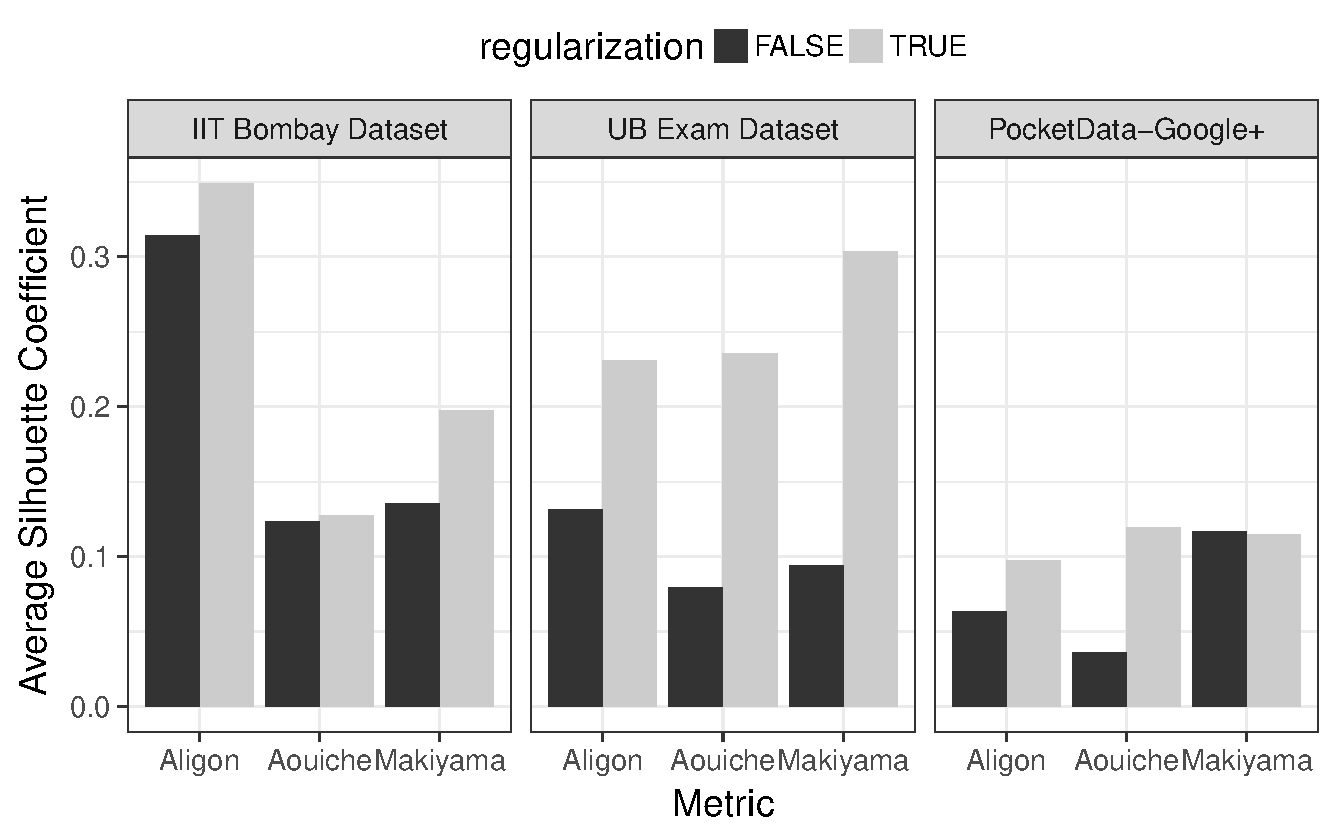
\includegraphics[width=\textwidth]{graphics/silhouette2}
        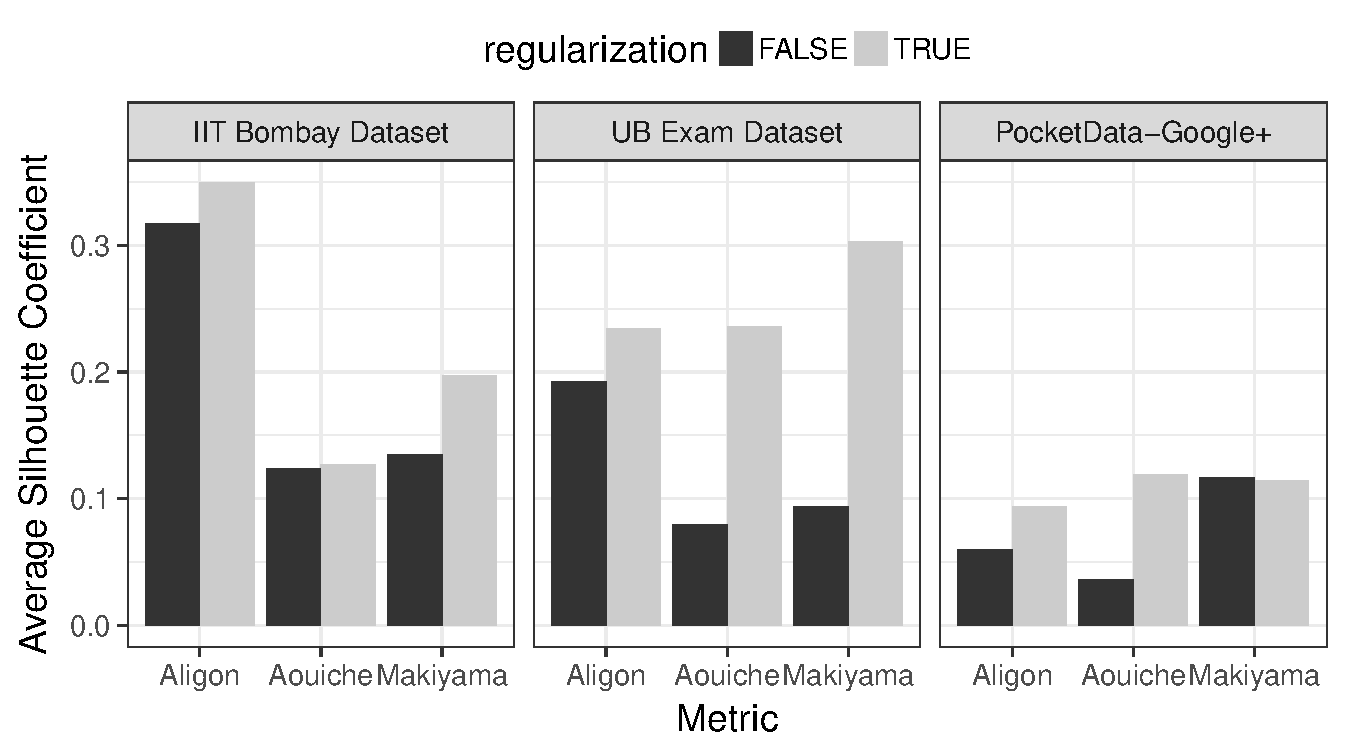
\includegraphics[width=\textwidth]{TKDE-QuerySimilarity/graphics/compare_silhouette}
        \caption{Average Silhouette Coefficient\\(\textit{larger} values are better)}
    \end{subfigure}%
    ~
    \begin{subfigure}[b]{0.48\textwidth}%{0.322\textwidth}
        \centering
        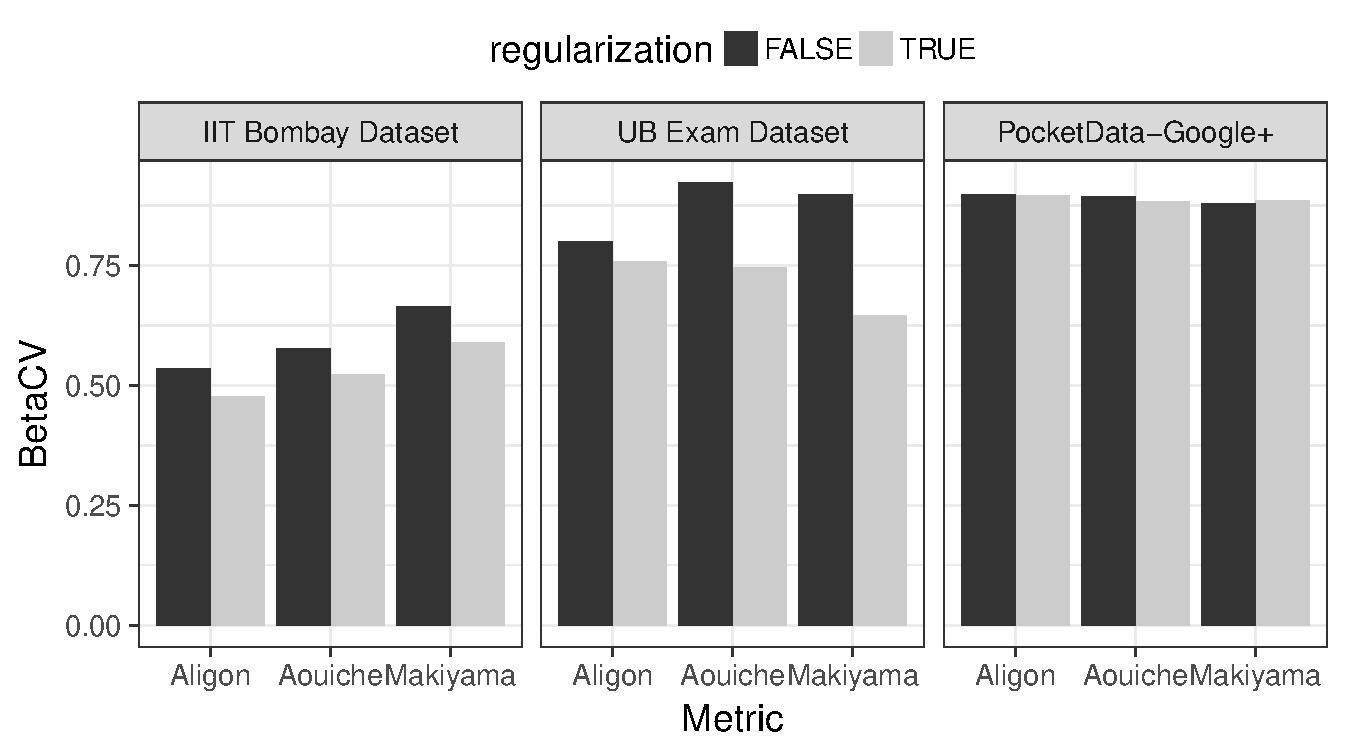
\includegraphics[width=\textwidth]{TKDE-QuerySimilarity/graphics/compare_betacv}
        \caption{BetaCV\\(\textit{smaller} values are better)}
    \end{subfigure}
    ~
    \begin{subfigure}[b]{0.48\textwidth}%{0.322\textwidth}
        \centering
        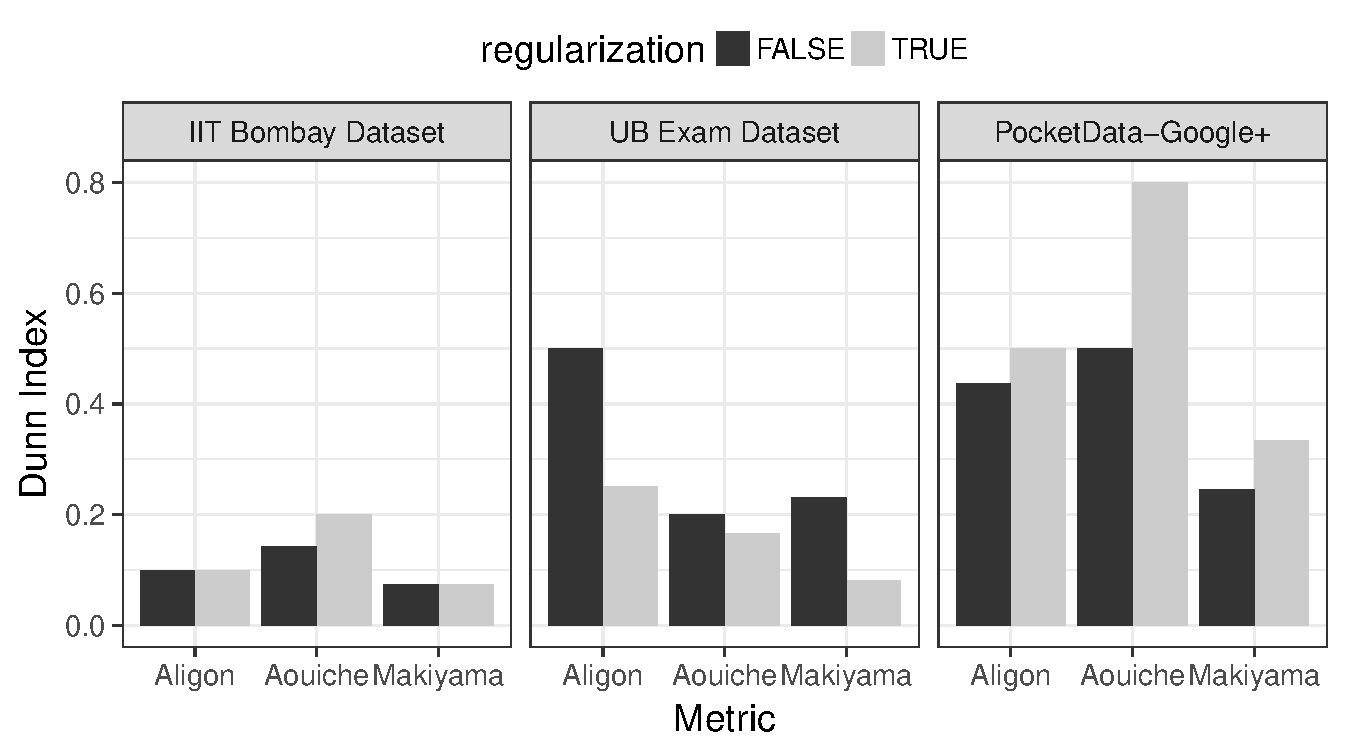
\includegraphics[width=\textwidth]{TKDE-QuerySimilarity/graphics/compare_dunn}
        \caption{Dunn Index\\(\textit{larger} values are better)}
    \end{subfigure}
    \caption{Clustering validation measures for each metric with and without regularization step}
    \label{fig:comparison2}
\end{figure*}

The black columns in Figure~\ref{fig:comparison2} show a comparison of three similarity metrics using each of the three quality measures (Average Silhouette Coefficient, BetaCV and Dunn Index).  
As can be seen in Figure~\ref{fig:comparison2}, Aligon seems to work the best for both IIT Bombay and UB Exam dataset while achieving second-best for PocketData-Google+ dataset under the Average Silhouette Coefficient measure. 
When considering BetaCV measure, Aligon also attains the best result for both IIT Bombay and UB Exam dataset while having comparable result for PocketData-Google+ dataset.
Aligon also performs well on the Dunn Index, coming in first on UB Exam dataset, and second-best for IIT Bombay and PocketData-Google+ dataset.
Especially given that the Dunn Index measures only worst-case performance, Aligon's metric seems to be ideal for our workloads.
This shows that even a fairly simple approach can capture task similarity well. 

\begin{figure*}[h!]
	\captionsetup[subfigure]{justification=centering}
    \centering
    \begin{subfigure}[b]{0.45\textwidth}%{0.32\textwidth}
        \centering
        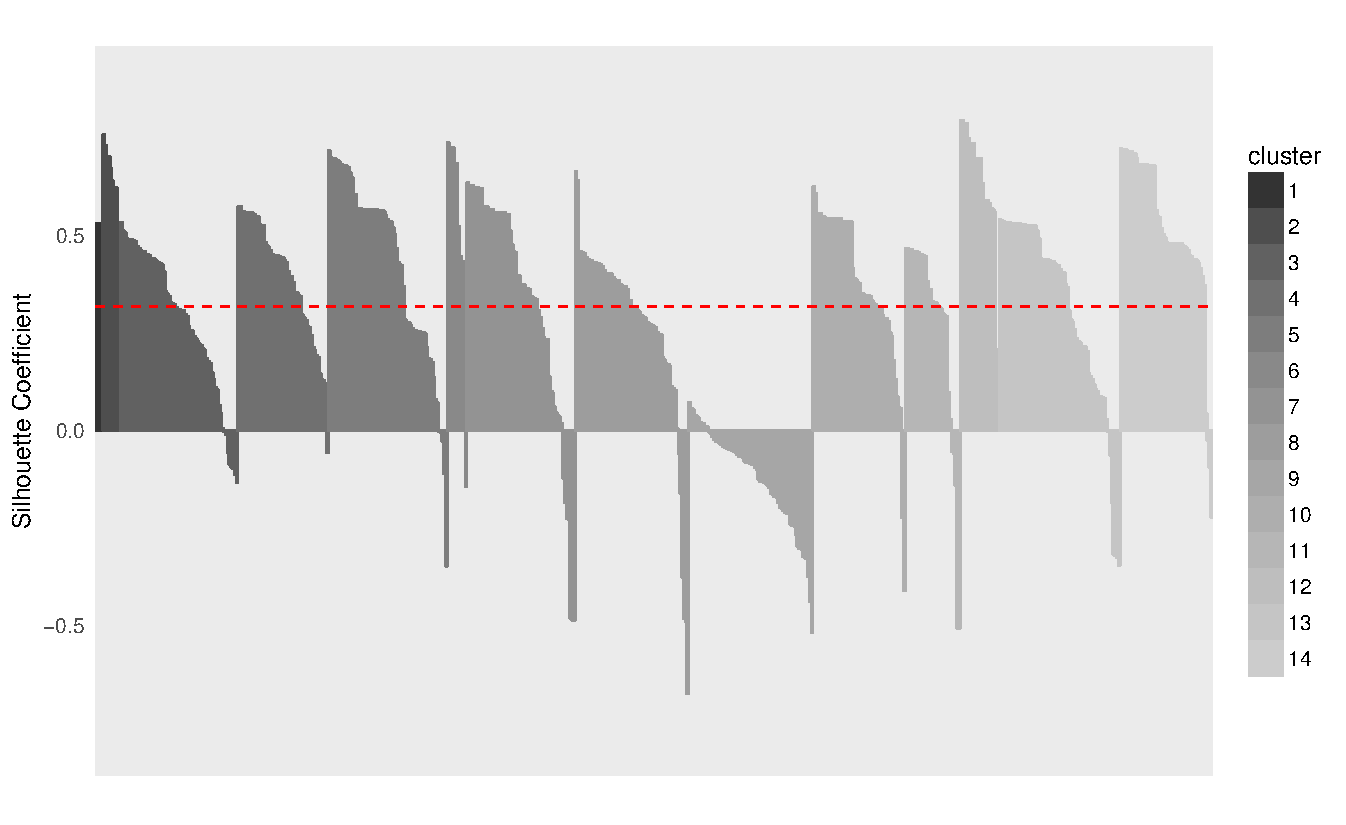
\includegraphics[width=\textwidth]{TKDE-QuerySimilarity/graphics/sil_bombay_Aligon}
		\caption{IIT Bombay dataset}
        \label{fig:sil_aligon:bombay}
    \end{subfigure}
    ~
    \begin{subfigure}[b]{0.45\textwidth}%{0.32\textwidth}
        \centering
        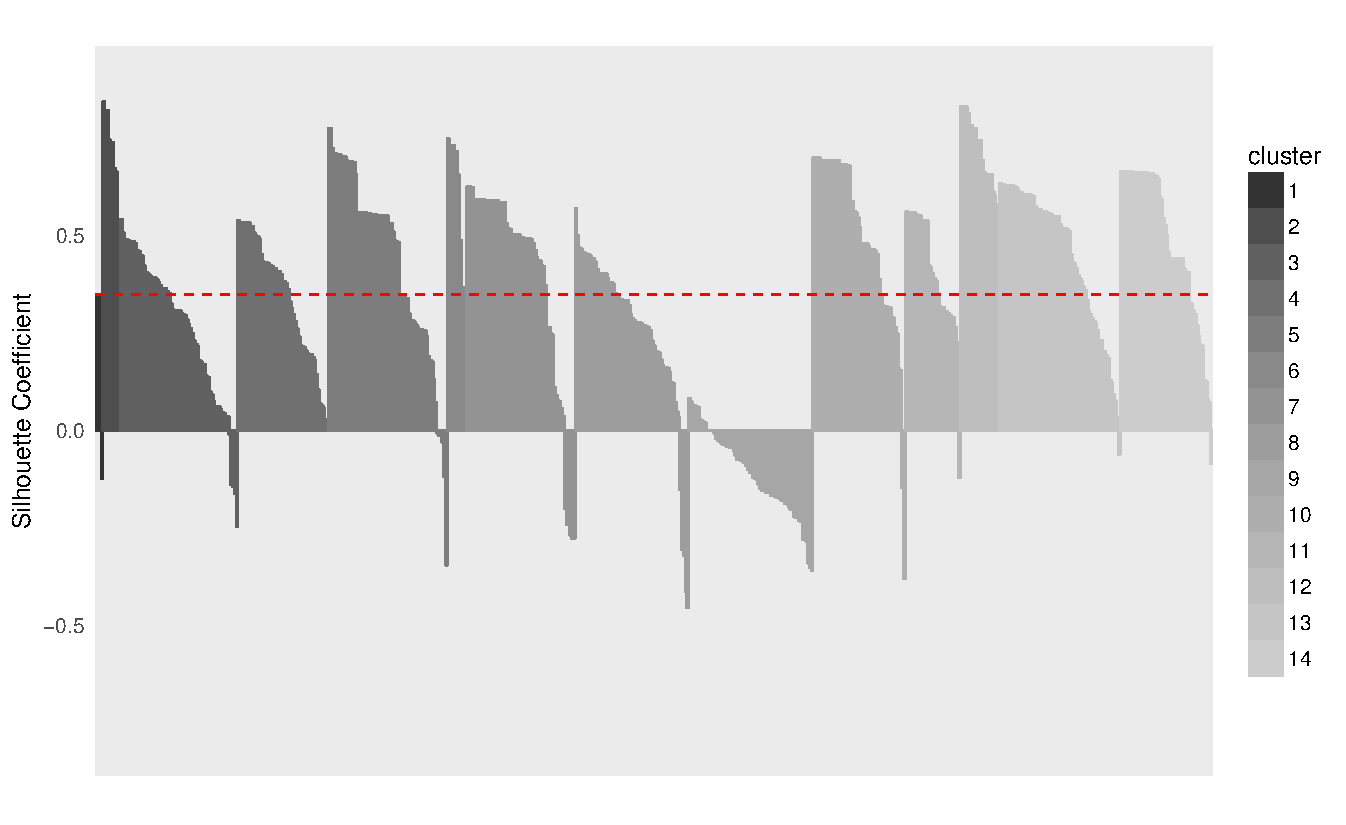
\includegraphics[width=\textwidth]{TKDE-QuerySimilarity/graphics/sil_bombay_Aligon_regularization}
		\caption{IIT Bombay dataset}
		\label{fig:sil_aligon:bombay_preprocess}
    \end{subfigure}
    \\
    \begin{subfigure}[b]{0.45\textwidth}%{0.32\textwidth}
        \centering
        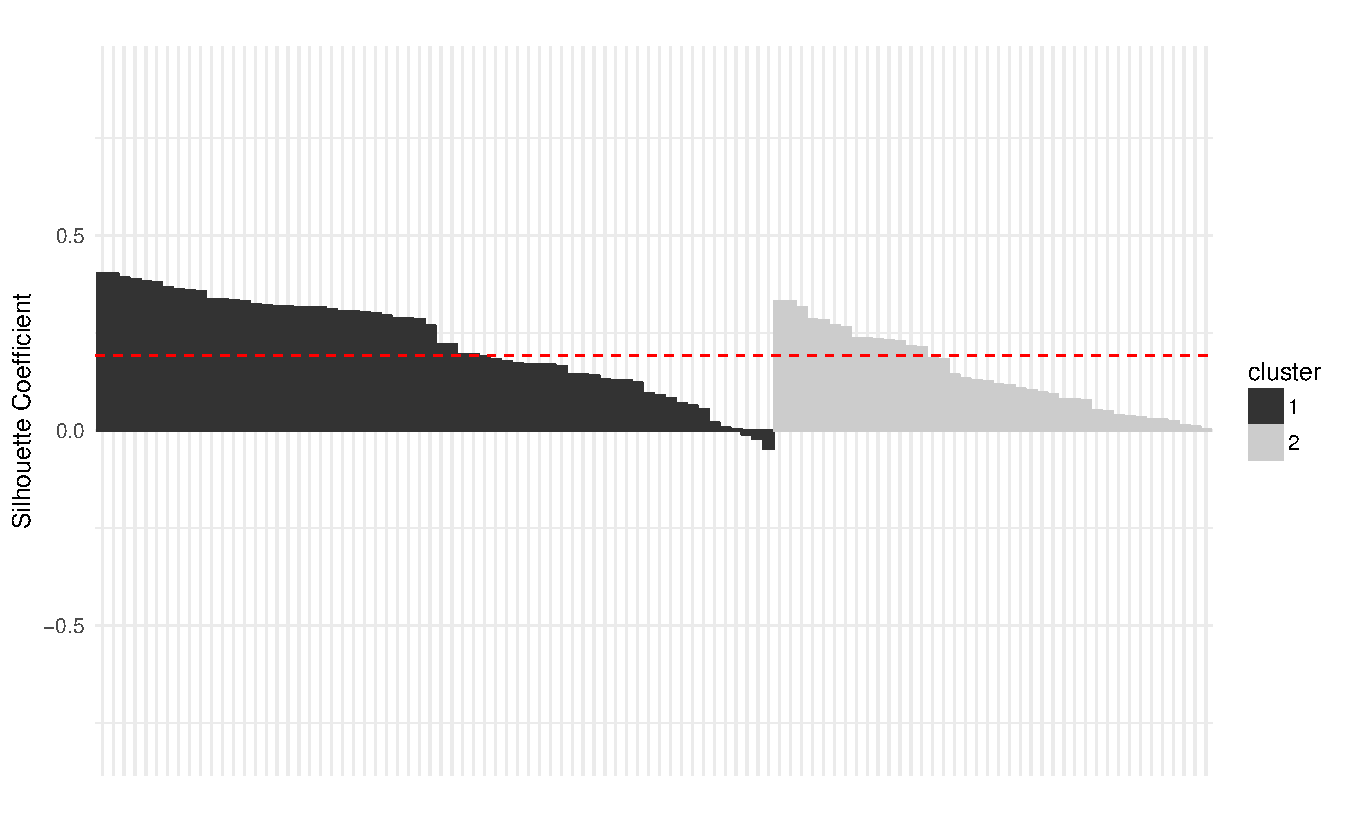
\includegraphics[width=\textwidth]{TKDE-QuerySimilarity/graphics/sil_ub_Aligon}
        \caption{UB Exam dataset}
        \label{fig:sil_aligon:local}
    \end{subfigure}
    ~
	\begin{subfigure}[b]{0.45\textwidth}%{0.32\textwidth}
        \centering
        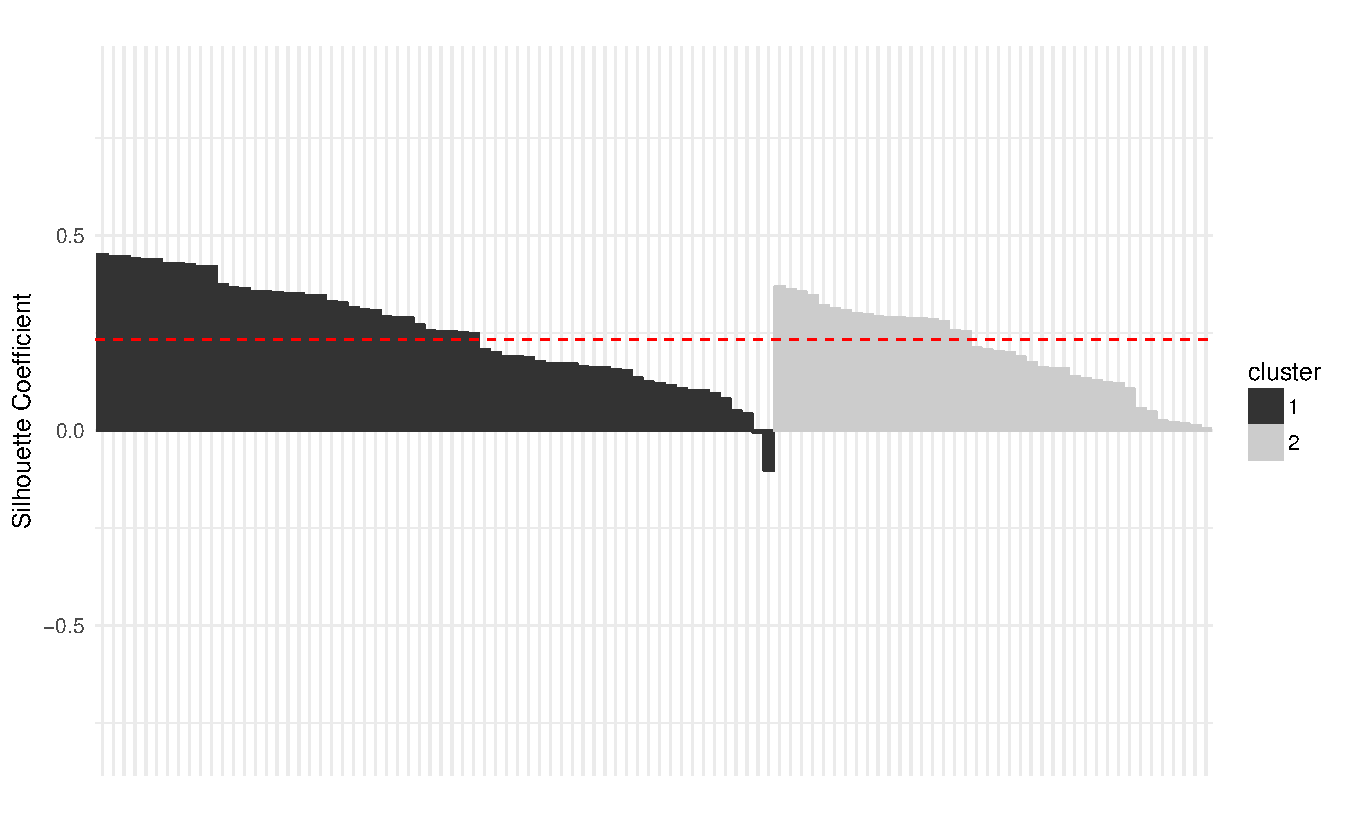
\includegraphics[width=\textwidth]{TKDE-QuerySimilarity/graphics/sil_ub_Aligon_regularization}
        \caption{UB Exam dataset}
        \label{fig:sil_aligon:local_preprocess}
    \end{subfigure}    
    \\
    \begin{subfigure}[b]{0.45\textwidth}%{0.32\textwidth}
        \centering
        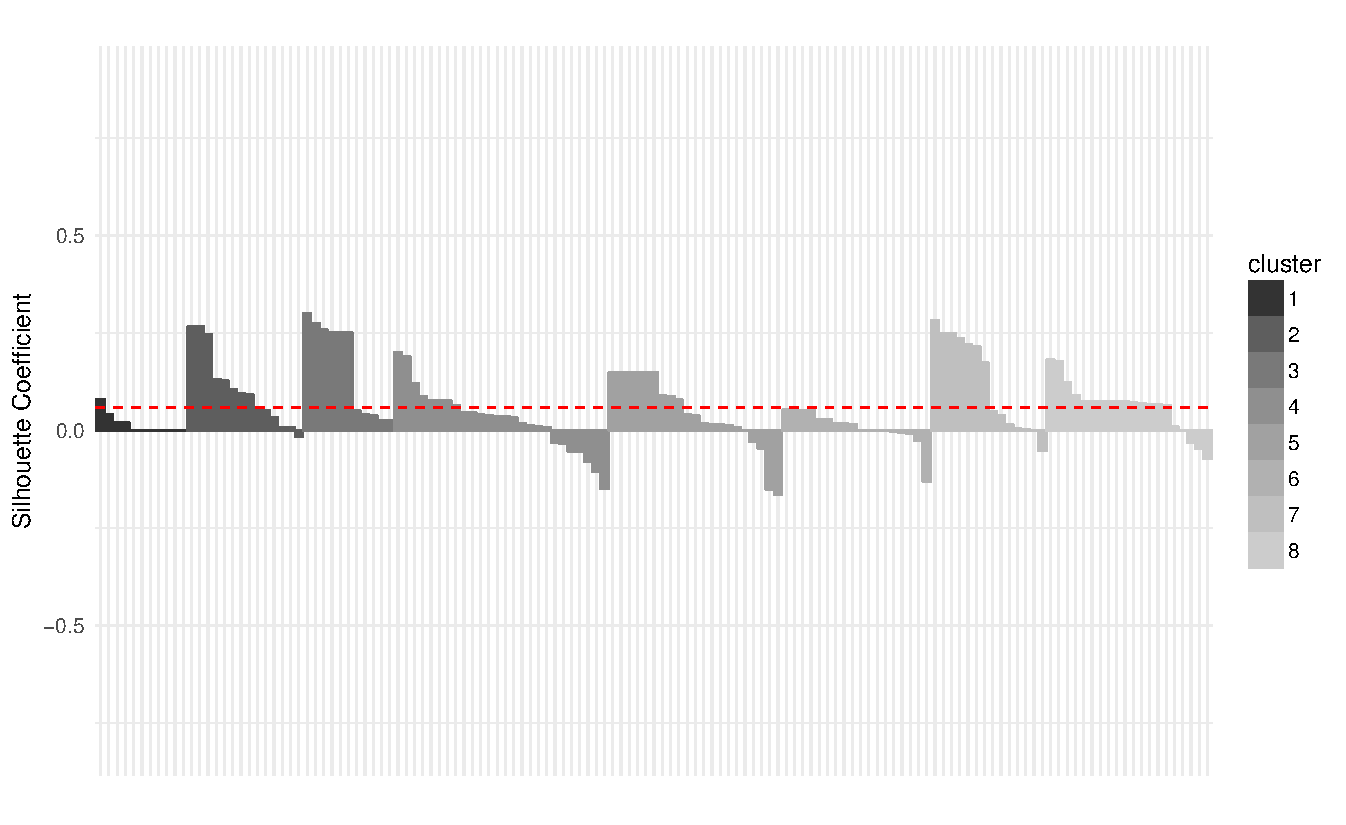
\includegraphics[width=\textwidth]{TKDE-QuerySimilarity/graphics/sil_googleplus_Aligon}
        \caption{PocketData-Google+ dataset}
        \label{fig:sil_aligon:googleplus}
    \end{subfigure}
    ~
    \begin{subfigure}[b]{0.45\textwidth}%{0.32\textwidth}
        \centering
        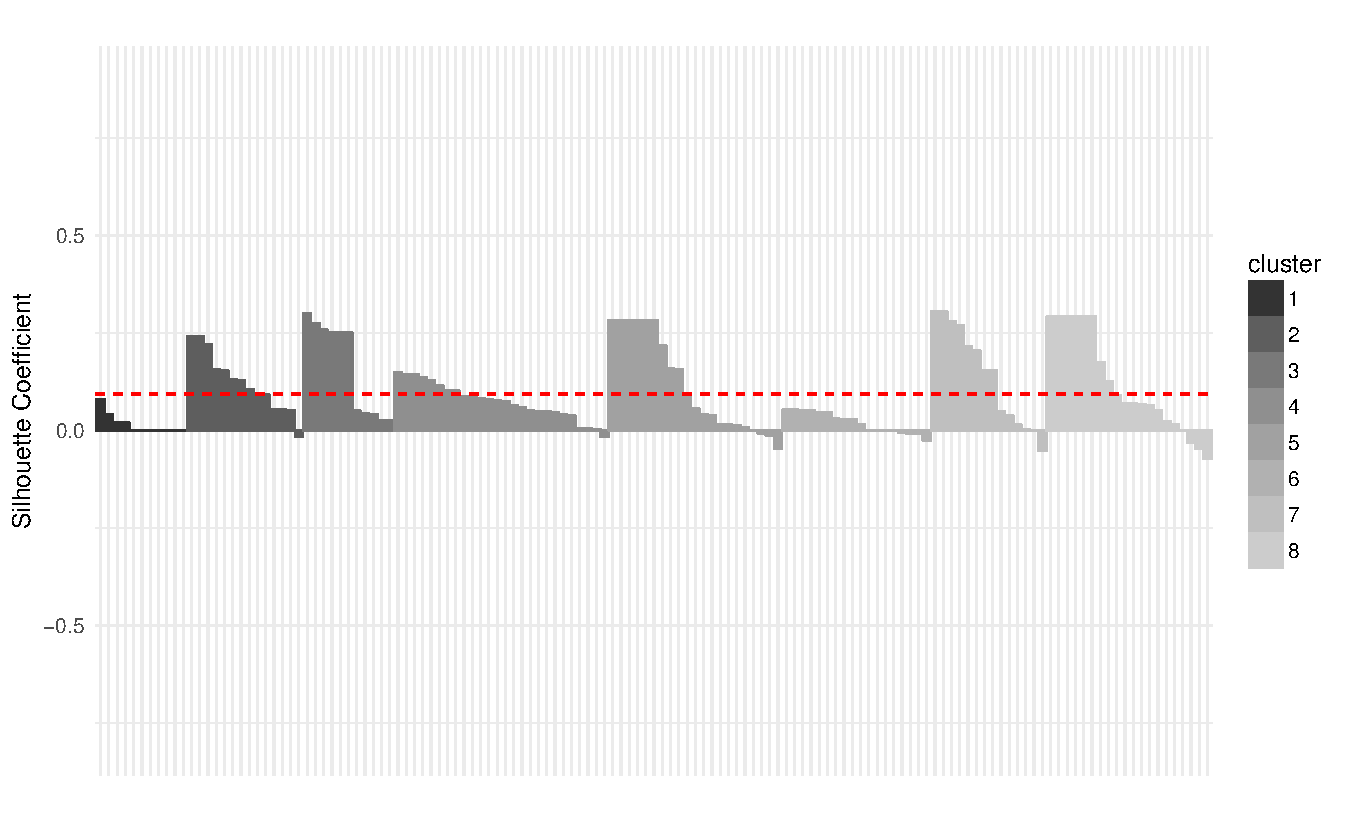
\includegraphics[width=\textwidth]{TKDE-QuerySimilarity/graphics/sil_googleplus_Aligon_regularization}
        \caption{PocketData-Google+ dataset}
        \label{fig:sil_aligon:googleplus_preprocess}
    \end{subfigure}
    \caption{Distribution of silhouette coefficients when using Aligon's similarity without regularization (a,c,e), and when regularization is applied (b,d,f)}
    \label{fig:sil_aligon}
    \label{fig:sil_aligon_preprocessed}
\end{figure*}

For a closer look of Aligon's similarity metric, Figure~\ref{fig:sil_aligon}(a,c,e) shows the distribution of Silhouette coefficients for each query and their respective tasks.   
Recall that the silhouette coefficient below 0 effectively indicates a query closer to another cluster than its own, or a query that would be mis-classified.  The further below zero, the greater the error.  
For the UB Exam dataset (Figure~\ref{fig:sil_aligon:local}), the majority of queries would have been successfully classified, and only a small fraction exhibit minor errors.
For the PocketData-Google+ dataset (Figure~\ref{fig:sil_aligon:googleplus}), there are some erroneous queries in cluster 4, 5 and 6 while cluster 1, 2, 3, 7 and 8 have very few errors.
For the Bombay dataset (Figure~\ref{fig:sil_aligon:bombay}), the distribution of errors varies.  
Cluster 1, 2, 4, 6, 12 and 14 exhibit virtually no error, while cluster 7, 8, and 9 exhibit particularly egregious errors.

\subsection{Evaluation of feature engineering}
\label{subsec:evaluation}
The effectiveness of regularization is evaluated by applying it to each of the three metrics described in Section~\ref{sec:background}.
The quality evaluation scheme is used to compare the quality of each measure both with and without feature engineering.

Figure~\ref{fig:comparison2} shows the values of three validation measures for each of the three similarity metrics, both with and without regularization.
As shown in Figure~\ref{fig:comparison2}, regularization significantly improves the Average Silhouette Coefficient and BetaCV measures for all similarity metrics except for the case of Makiyama similarity metric with PocketData-Google+ dataset.
The Dunn index is relatively unchanged or little improved for the IIT Bombay and PocketData-Google+ dataset and shows slight signs of worsening with regularization on the UB Exam dataset. To understand the reason of worse Dunn Index, Figure~\ref{fig:sil_aligon:local} (original) is compared with Figure~\ref{fig:sil_aligon:local_preprocess} (with regularization). 
The Silhouette Coefficient for answers that are originally positive in each question are considerably increased, and for answers that are originally negative (regarded erroneous) are even more decreased as a result of regularization, since it reduces the query structure diversity which leads to separating queries better.
In other words, for erroneous answers with negative Silhouette Coefficients, distance metrics like Aligon distinguish them further apart from answers with positive Silhouette Coefficients after regularization. 
Since erroneous answers are treated as the `worst cases' for each question, the Dunn Index which measures worst case performance naturally gets worse.

\subsubsection{Per-Query Similarity}
Figure~\ref{fig:sil_aligon_preprocessed}(b,d,f) shows the distributions of silhouette coefficients for the Aligon similarity metric after regularization is applied.  
For IIT Bombay dataset, comparing against Figure~\ref{fig:sil_aligon:bombay} there is a slight improvement at the tail end of clusters 9, 11, 12, 13 and 14 --- several of the negative coefficients have been removed.  
Furthermore, positive matches have been improved, particularly for cluster 7, 9, 10, 12 and 13.  
Finally, there has been a significant reduction in the degree of error in cluster 10.  
Cluster 10 is a particularly egregious case of aliasing, as the correct answer involves two self-joins in the same query.
As a result, aliasing is a fundamental part of the correct query answer, and our rewrites could not reliably create a uniform set of alias names.
In the UB Exam and PocketData-Google+ datasets, the improvement provided by regularization can be seen for queries with both positive and with negative values of $s(i)$.


\subsection{Case Study}
As part of the analysis, empirical explanations for query errors are provided by manual work, in particular for queries where $s(i) < 0$ for all three similarity metrics. 
Namely, queries that are too far apart from the clusters they belong are manually examined, and the reasons for mis-classification are categorized. 
We then investigate how the regularization process particularly affect these queries. 

Almost all of these egregiously mis-classified queries appear in the IIT Bombay dataset, the distribution of which is summarized in Table~\ref{tab:errorsources}.
The PocketData-Google+ dataset includes no egregiously mis-classified queries, while the UB Exam dataset includes only one such query (which tagged as a case of \textbf{Contextual equivalence}).
Each egregiously mis-classified query is tagged with an explanation that justifies why the query has a low s(i). 
Tags were drawn from the following list:

\smallskip
\tinysection{Ground-truth error} A student's response to the question may have been legitimately incorrect. This is a query that is correctly classified as an outlier.
For example: 
{\footnotesize
\begin{verbatim}
SELECT *
FROM (SELECT id, name, time_slot_id
 FROM (SELECT *
  FROM (SELECT *
   FROM student
    NATURAL JOIN takes) b1) a, section
   WHERE a.course_id = section.course_id) a1
\end{verbatim}
}
This query was attempting to complete the task \textit{``Find the ID and names of all students who have (in any year/semester) taken two courses in the same timeslot.''}

\smallskip
\tinysection{Nested subquery} A student's response is equivalent to a legitimately correct answer but uses nested subqueries such that a heuristic distance metric cannot recognize.
For example: 
{\footnotesize
\begin{verbatim}
SELECT id, name FROM student
WHERE id IN (SELECT DISTINCT s.id
 FROM (SELECT * FROM takes NATURAL JOIN section) s,
  (SELECT * FROM takes NATURAL JOIN section) t
 WHERE s.id = t.id
  AND s.time_slot_id = t.time_slot_id
  AND s.course_id <> t.course_id)
\end{verbatim}
}

Here, the subquery nesting structure is significantly different from other queries for of the same question.

\smallskip
\tinysection{Aliasing} Aliasing (e.g., \texttt{AS} in SQL) breaks a distance metric that relies on attribute and relation names.
For example:
{\footnotesize
\begin{verbatim}
SELECT DISTINCT student.id, student.name
FROM student, takes, section AS a, section AS b
WHERE student.id = takes.id
  AND takes.course_id = a.course_id
  AND takes.course_id = b.course_id
  AND a.course_id <> b.course_id
  AND a.time_slot_id = b.time_slot_id
\end{verbatim}
}

The student's use of \texttt{a} and \texttt{b} make this query hard to distinguish from other queries that may use other names for the attributes.

\smallskip
\tinysection{Insufficient features} Relevant query components are not sufficiently captured as features for a heuristic distance metric to distinguish between answers from sufficiently similar questions.

\smallskip
\tinysection{Too many features} Irrelevant query components create redundant features that artificially increase the distance between the query and cluster center.
For example:
{\footnotesize
\begin{verbatim}
SELECT DISTINCT student.name, takes.id, 
                s1.course_id, s2.course_id
FROM section AS s1, section AS s2, takes, student
WHERE takes.course_id = s1.course_id
  AND s1.course_id <> s2.course_id
  AND s1.time_slot_id = s2.time_slot_id
  AND s1.semester = s2.semester
  AND s1.year = s2.year
  AND takes.sec_id = s1.sec_id
  AND s1.semester = takes.semester
  AND s1.year = takes.year
  AND student.id = takes.id
  AND s2.time_slot_id = s2.time_slot_id
  AND takes.sec_id = s2.sec_id
  AND s2.semester = takes.semester
  AND s2.year = takes.year
\end{verbatim}
}

\smallskip
\tinysection{Contextual equivalence} Establishing query equivalence to properly clustered queries requires domain-specific knowledge not available to the distance metric (e.g. attribute uniqueness).
For example:
{\footnotesize
\begin{verbatim}
SELECT student.id, student.name
FROM student
WHERE student.id
  IN (SELECT takes.id
    FROM takes, section
    WHERE takes.course_id = section.course_id
      AND takes.sec_id = section.sec_id
      AND takes.semester = section.semester
      AND takes.year = section.year
    GROUP BY takes.id,
        takes.semester,
        takes.year,
        section.time_slot_id
    HAVING count(*) > 1)
\end{verbatim}
}

\begin{table}[h!]
%\vspace{-3mm}
\centering
\begin{tabular}{ccccccc}
\toprule
 \textbf{\begin{tabular}[c]{@{}c@{}}Cause\end{tabular}} & \textbf{\begin{tabular}[c]{@{}c@{}}Erroneous \\queries \\ Without \\ Regularization\end{tabular}} & 
 \textbf{\begin{tabular}[c]{@{}c@{}}Erroneous \\queries \\ With \\ Regularization\end{tabular}}\\
 \midrule
 All queries & 33 (100\%) & 27 (100\%)\\% & 1 (100\%) & 1 (100\%) & 0 (100\%)& 0 (100\%)\\  
 Ground-truth quality & 14 (42.4\%) & 14 (51.8\%)\\% & 0 (0\%) & 0 (0\%) & 0 (0\%) & 0 (0\%)\\ 
 Nested subquery & 7 (21.2\%) & 5 (18.5\%)\\% & 0 (0\%) & 0 (0\%) & 0 (0\%) & 0 (0\%)\\ 
 Aliasing & 8 (24.2\%) & 5 (18.5\%) \\%& 0 (0\%) & 0 (0\%) & 0 (0\%) & 0 (0\%)\\ 
 Insufficient features & 2 (6.0\%) & 1 (3.7\%)\\% & 0 (0\%) & 0 (0\%) & 0 (0\%) & 0 (0\%)\\ 
 Too many features & 1 (3.0\%) & 1 (3.7\%) \\%& 0 (0\%) & 0 (0\%) & 0 (0\%) & 0 (0\%)\\ 
 Contextual equivalence & 1 (3.0\%) & 1 (3.7\%)\\% & 1 (100\%) & 1 (100\%) & 0 (0\%) & 0 (0\%)\\
 \bottomrule
\end{tabular}
\vspace{-2mm}
\caption{Empirical error reasons for IITBombay Dataset}
\label{tab:errorsources}
%\vspace{-3mm}
\end{table}

Table~\ref{tab:errorsources} shows the primary reasons why these queries could not be classified correctly. 
Note that there may be more than one reason for a query to be placed in a different cluster, but in Table~\ref{tab:errorsources}, only the empirically determined primary reason is given.

Many of the queries with low silhouette coefficients are identified as incorrect answers for the task given. 
These answers directly affect the ground-truth quality, therefore reduce the average silhouette coefficient. 
Another reason for erroneous queries with low silhouette coefficients is because of aliasing. 
Although it is convenient for user to use aliases in the query to refer to a particular item, it is difficult for a machine to approximate the tasks the query authors are trying to accomplish since different query authors have different ways to name particular items in the query. 
This problem is particularly prevalent in question 9 of the IIT Bombay dataset.

Although the distribution of the error reasons are expected to change, all the tags provided in this section can generically be applied to other query logs given a ground-truth. 
The regularization method cannot be expected to fix errors originating from mis-classifications in ground-truth since they do not actually share any similarities with the cluster. 

After the regularization process, the silhouette coefficient under all three similarity metrics for each query is computed again and the result yields an 18\% overall reduction in number of erroneous queries ($s(i) < 0$)  in the IIT Bombay dataset. 

\subsection{Analysis of regularization by module}
\label{subsec:modules}
In subsection~\ref{subsec:evaluation}, the overall effect of regularization on query similarity is analyzed.  
However, as described in Section~\ref{sec:system}, regularization is composed of many different transformation rules.  
In this experiment, these rules are grouped into four separate modules before their impact on the clustering quality is inspected. 
One may observe that Commutative Operator Ordering is guaranteed to provide benefit in structure similarity comparison, hence it is included in all four modules. 
In addition, there are dependencies between rules that require them to operate one before another. 
For example, one should better apply Syntax Desugaring and then DNF Normalization to simplify the boolean expression in WHERE clause before OR-Union Transformation.
As another example, Exists Standardization should better be applied on nested sub-queries before we de-correlate them using Nested Query De-correlation.
As a result, the rules are grouped from Section~\ref{sec:system} into four modules:
\begin{enumerate}
\item \textit{Naming}: \textbf{Canonicalize Names and Aliases}
\item \textit{Expression Standardization}: \textbf{Syntax Desugaring}, \\\textbf{Exists~Standardization}, \textbf{DNF~Normalization}, \\\textbf{Nested~Query~Decorrelation}, \textbf{OR-Union~Transform}
\item \textit{FROM-Nesting}: \textbf{Flatten FROM-Nesting}
\item \textit{Union Pullout}: \textbf{OR-UNION Pullout}
\end{enumerate}
\textbf{Commutative Operator Ordering} is included in all modules.

Figure~\ref{fig:module} provides a comparison of each module in regularization. 
From this figure, one can observe that, since students use different names/aliases for their convenience when constructing queries, the \textit{Naming} module is the most effective one in terms of improving clustering quality for IIT Bombay and UB Exam datasets. 
On the other hand, for PocketData-Google+ dataset, names are already canonicalized as they are machine-generated. 
In this case, \textit{Expression Standardization} seems to be the most effective module, especially when using Aligon or Aouiche as similarity metric. 
In PocketData-Google+ dataset, referred tables and boolean expressions in the queries are both informative in distinguishing between different query categories or clusters. For this reason, Makiyama similarity metric which considers both works well even without regularization while Aligon and Aouiche can get commensurate performance only after applying \textit{Expression Standardization} module. 

Note that in Figure~\ref{fig:module}, \textit{Expression Standardization} makes Average Silhouette Coefficient worse in some cases for IIT Bombay and UB Exam data sets. 
The performance degradation is majorly due to \textit{feature duplication}. 
More specifically, consider the example query with \textit{Expression Standardization}.
\begin{example}
Syntax Desugaring with OR-UNION transform
{\footnotesize
\begin{enumerate}
\item\begin{verbatim}
SELECT name FROM usr WHERE 
rank IN {'admin','normal'}
\end{verbatim}
\item\begin{verbatim}
SELECT name FROM usr WHERE 
rank = 'admin' OR rank = 'normal'
\end{verbatim}
\item\begin{verbatim}
SELECT name FROM usr
WHERE rank = 'admin'
UNION
SELECT name FROM usr
WHERE rank = 'normal' 
\end{verbatim}
\end{enumerate}
}
\end{example}
Query (1) is transformed into (2) by syntax~desugaring and then into (3) by OR-UNION~Transform. From (1) to (2), feature \texttt{WHERE rank} has been replicated; From (2) to (3), features \texttt{SELECT name} and \texttt{FROM usr} have been duplicated. For expressions of the form: \texttt{X IN} $\{x_1,x_2,\dots,x_n\}$, feature duplication becomes dominant when $n$ grows large. 
In Figure~\ref{fig:module}, Aligon and Makiyama suffer from feature duplication brought by~\textit{Expression Standardization} in some cases while Aouiche does not. 
Because Aouiche records feature existence instead of occurrence in its vector. 
Although in some cases such as this, simply replacing feature occurence with existence solves the problem of feature duplication, feature occurence can also be a good indicator for the interests of the query. 
It is believed that this problem can be addressed with exploration of feature weighting strategies. 
Therefore, the problem of feature duplication will be further explored as a part of feature weighting strategies in our future work.

\begin{figure*}[h!]
    \vspace*{-2mm}
    \centering
    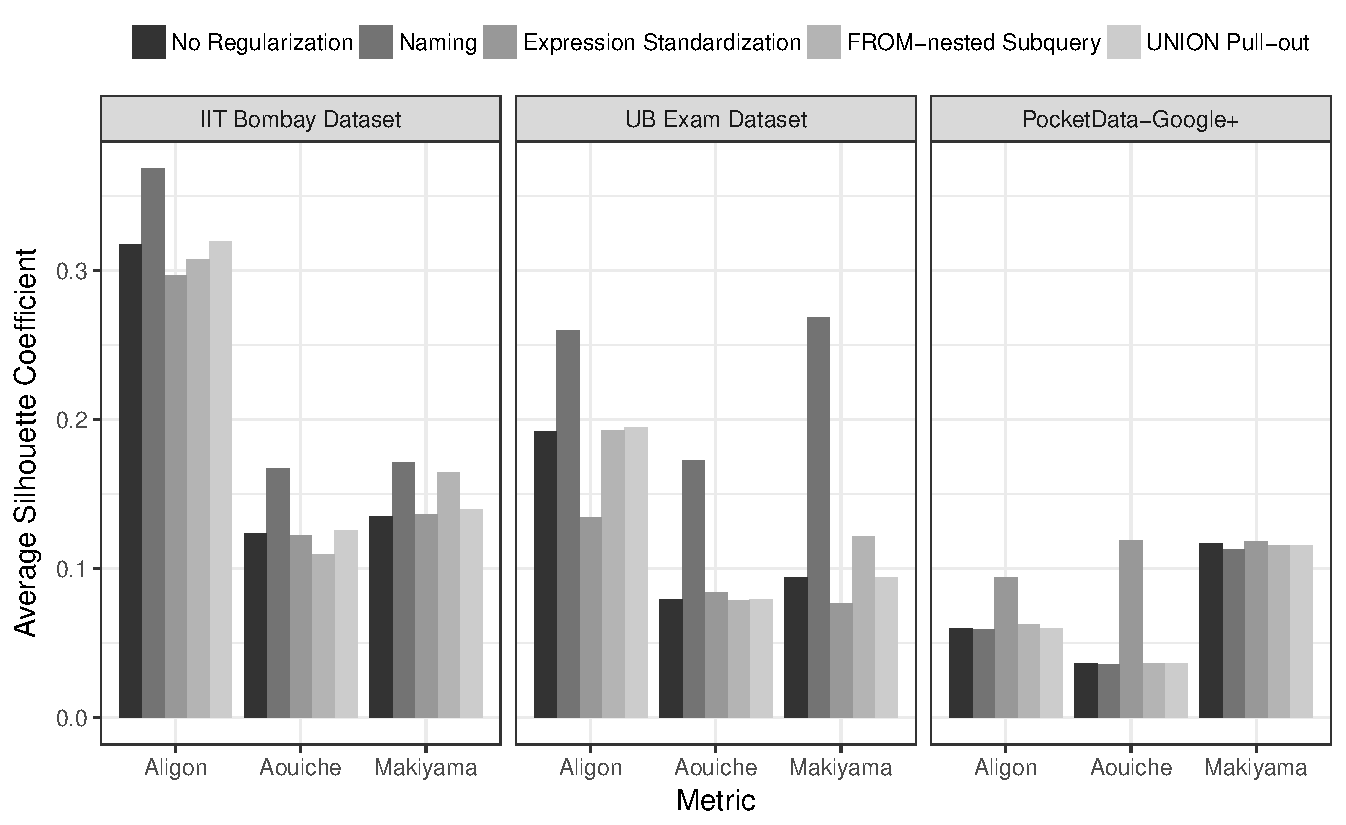
\includegraphics[width=0.70\textwidth]{TKDE-QuerySimilarity/graphics/module}%[width=\columnwidth]{graphics/module}
	\caption{Effect of each module in regularization}
    \label{fig:module}
    %\vspace*{-4mm}
\end{figure*}



\section{Discussion}
\label{sec:discussion}
% !TEX root = ../paper.tex
%This paper presents the first steps for \sysname{}.
We have reviewed several similarity metrics for clustering queries and focused on three syntax-based methods that offer an end-to-end similarity metric. The advantage of this preference is that, syntax-based methods do not require access to the data in the database or database properties. Considering that only logs are usually transferred between organizations, and requiring access to the data for investigations can cause privacy violations, we preferred focusing on the syntax-based approach.

The survey we performed shows that most of the metrics make use of selection and join operations in the queries and consider them as the most important items for similarity calculation. Group-by aggregate follows them closely while projection items take the third most important item set. There are other possible feature sets that can be used, such as tables accessed or the abstract syntax tree (AST) of a query, but these feature sets are generally overlooked.

%We have surveyed and measured the evaluation of query similarity metrics for clustering similar queries together and picked three methods that offer an end-to-end similarity metric. The survey shows that most of the metrics make use of selection and join predicates and consider them the most important items for similarity comparison. Group-by predicates follows them closely while projection items take the third most important item set. There are other possible feature sets that can be used in queries like the tables accessed or the AST of a query, but these feature sets are generally overlooked.

%As shown in Figure~\ref{fig:comparison1}, apart from the Dunn index value for IIT Bombay dataset, Aligon \textit{et al.}~\cite{aligon2014similarity} performs the best amongst the surveyed methods.
% All the approaches surveyed can provide the user with an immediate view on the quality of their clustering. 
%The success of this method can be attributed to the choice of the feature set: selection, joins, group by and projection items separately have their own weightings in the general calculation of the similarity.
Although Aouiche \textit{et al.}~\cite{aouiche2006}
%have a similar strategy; making
make use of the most important features selection, joins, and group-by items, they don't utilize the number of times an item appears, or after the parsing, they don't consider what kind of feature an item is. This means, it does not matter if a query has \texttt{rank} column in group-by, and the other one has \texttt{rank} column in selection; they are considered the same. Makiyama \textit{et al.}~\cite{makiyama2015text}, on the other hand, follow Aligon \textit{et al.}~\cite{aligon2014similarity} in separating the different features, and improves on it by making use of appearance count of items. However, while trying to make use of every item like \texttt{FROM} and \texttt{Order-By} predicates, they consider these low priority predicates with same importance as the selection and join predicates.

Makiyama \textit{et al.}~\cite{makiyama2015text} use a more complete structure of the query AST, hence when the query is simple like in the PocketData-Google+ dataset, this technique can be slightly better.
However, for a complex query with redundant features, mixing features captured from various components of a query without proper feature re-weighting will essentially decrease the weight of features that are more informative.
Hence, in student exam datasets, we can observe that Aligon \textit{et al.}~\cite{aligon2014similarity} is better than the others while in PocketData-Google+ dataset, Makiyama \textit{et al.}~\cite{makiyama2015text} is better.

We could further improve these methods by making use of the abstract syntax tree (AST) of a SQL statement.
As a declarative language, the AST of a SQL statement acts as a proxy for the task of the query author.
This suggests that a comparison of ASTs can be a meaningful metric for query similarity.
For instance, we can group a query $Q$ with other queries that have nearly (or completely) the same AST as $Q$.
This structural definition of task has seen substantial use already, particularly in the translation of natural language queries into SQL~\cite{li2015NLPI}.
For two SQL queries $Q_1$ and $Q_2$, one reasonable measure might be to count the number of connected subgraphs of $Q_1$ that are isomorphic to a subgraph of $Q_2$.  
Subgraph isomorphism is NP-complete, but a computationally tractable simplification of this metric can be found in the Weisfeiler-Lehman (WL) Algorithm~\cite{WL2011, kul2016ettu}.

As can be seen in Tables~\ref{tab:xdata} and \ref{tab:ub_exam}, as the complexity or difficulty of the question increases, the number of distinct queries also increases, i.e., students find different ways to solve the same problem.
Especially, in Table~\ref{tab:ub_exam}, no two students answer a question using the same structure.
This phenomenon motivates the need for regularization in comparing SQL queries.
As the complexity of the query increases, the possible ways to create the query to achieve the same task increase.
Figure~\ref{fig:comparison2} shows that our assumption that regularizing queries will improve overall clustering quality is correct.
Our proposed feature engineering scheme improves the overall clustering quality of all three metrics on all three datasets, including both human- and machine-generated queries.

%One caveat is that regularization is only suitable for query comparison purpose as some of its transformations do not retain equivalence.
%In addition, once a nested sub-query is flattened and merged with its parent, aliases in the parent query pointing to it become invalid.
%At the same time, names across different query bodies are merged and name uniqueness is not guaranteed any more.
%Skewed names in the query will make query comparison error-prone.

%Although we run our experiments on a multi-core server, our implementations are single-threaded.
%We believe that modifying our algorithms to run parallel can significantly decrease the running time.

%Hence we apply a recommended step before regularization that renames all entities in the query containing aliases. 

%In Section~\ref{sec:WL}, we introduce a new similarity metric that is based on the feature extraction scheme based on the Weisfeiler--Lehman test of isomorphism on graphs where we make use of query ASTs instead of atomic features. Even with this naive approach, the performance of the metric is competitive with the metrics surveyed in this paper as can be seen in Figure~\ref{fig:comparison3}. The quality is further improved with the regularization scheme we proposed as shown in Figure~\ref{fig:comparison4}.  Furthermore, the algorithm can be benefit greatly from feature weighting (e.g. appointing higher weights to the features created from selection and joins) and dimensionality reduction with PCA, ICA or other feature selection techniques. Just like Makiyama \textit{et al.}~\cite{makiyama2015text}, we create many unimportant features along with the important ones, and feature selection can improve the accuracy of the metric greatly.


\section{Application Scenarios}
\label{sec:scenarios}
%!TEX root = ./sections/1-intro.tex
In this section, three scenarios are provided where the clustering scheme coupled with the proposed regularization is applicable:

The first one is, \textit{Jane the DBA} where she takes on the task of improving database performance.
After performing the straightforward database indexing tasks, she would need to select candidate \textit{views}, which are virtual tables defined by a query.
They allow querying just like tables by pre-fetching records from existing tables. 
Constructing a view for a frequent complex join operation can increase querying performance of the database substantially.
To find the ideal views, Jane first clusters similar queries together to see what kinds of queries are more frequent.
Making the most frequent complex query types faster by creating views of them could improve database performance substantially~\cite{aouiche2006, aligon2014similarity}. 

The second one is, \textit{Jane the security auditor} where she suspects that there is a person who leaks classified information from her organization.
She can choose to investigate database access patterns along with other strategies which would involve query clustering~\cite{Sun2016}.
After identifying the query clusters, she can partition the queries by the department or role to get the intuition about which departments and roles \textit{normally} utilize what part of the database.
She can detect the \textit{outliers} from that behavior in order to determine the suspects for further investigation.

Lastly, \textit{Jane the researcher} where needs to investigate the properties of the SQL query dataset that she is going to use for her research.
One of the new graduate students in her team clusters the queries, and provides her with the clustering assignments of each query.
She doubts the quality of the clustering performed, and wonders if the clustering operation could be performed better.

Having a \textit{better} clustering of queries would potentially enhance the quality of her work in all of the examples given above.
Also, works cited in this section~\cite{aouiche2006, aligon2014similarity, Sun2016}, along with many others can benefit from the framework described in this chapter.


\section{Conclusion and Future Work}
\label{sec:conclusion}
% !TEX root = ../paper.tex
The focus of this work is to understand and improve similarity metrics for SQL queries relying on query structure to be used to cluster queries. 
We described a quality evaluation scheme that captures the notion of query task using student answers to query-construction problems and a real-world smartphone query load.
We used this scheme to evaluate three existing query similarity metrics.
We also proposed a feature engineering technique for standardizing query representations.
Through further experiments, we showed that different workloads have different characteristics and no one similarity metric surveyed was always good. 
The feature engineering steps provided an improvement across the board because they addressed the error reasons we identified. 

The approaches described in this article only represent the first steps towards tools for summarizing logs by tasks.
Concretely, we plan to extend our work in several directions:
First, we will explore new feature extracting mechanisms like the Weisfeiler-Lehman framework~\cite{kul2016ettu}, feature weighting strategies and new labeling rules in order to capture the task behind logged queries better.
Second, we will introduce the temporal order of the log to increase the query clustering quality. In this article, we focused on query structures to improve clustering quality. Exploring the inter-query feature correlation based on query order can be used to summarize query logs in addition to clustering.
Third, we will examine user interfaces that better present clusters of queries --- Different feature sorting strategies in Frequent Pattern Trees (FP Trees)~\cite{han2004mining} in order to help the user distinguish important and irrelevant features, for example.
Lastly, we will investigate the temporal effects on query clustering. 
